\documentclass[format=acmsmall,screen]{acmart}
%% \settopmatter{printfolios=true,printccs=false,printacmref=false}

%% CJK setting
\usepackage{xeCJK}
\setCJKmainfont{SimSun}
\punctstyle{banjiao}

\usepackage{booktabs} % For formal tables
\usepackage{longtable}
\usepackage{tabu}
\usepackage{alltt}
\usepackage{microtype}
\usepackage{fancyvrb}
\usepackage[utf8]{inputenc}
\usepackage{acmshepherd}

\usepackage{natbib}
\citestyle{acmauthoryear}



%% Paper history
%% Not sure where we got this from, but the HOPL editors ended asking it be
%% removed ;-)
%% \received{August 2018}
%% \received[Revised]{August 2019}
%% \received[Final]{March 2020}
%%
%% Preliminary Chinese translation by Yue Yi <includeyy123@gmail.com>:
%% https://egh0bww1.com/posts/2023-05-21-37-tr-evolution-of-emacs-lisp

%% While Richard prefers "Emacs Lisp" I find it unnecessarily verbose
%% and much prefer "Elisp" which is also very widely used.
\newcommand \Elisp {Emacs Lisp}
\newcommand \MAlign [1] {\begin{array}{@{}l@{}}#1\end{array}}
\newcommand \TAlign [1] {\begin{tabular}{@{}l@{}}#1\end{tabular}}
\newcommand \id[1] {\textrm{\textsl{#1}}}

\hyphenation{na-me-spa-ce}

%%% The following is specific to HOPL '20 and the paper
%%% 'Evolution of Emacs Lisp'
%%% by Stefan Monnier and Michael Sperber.
%%%
\setcopyright{rightsretained}
\acmPrice{}
\acmDOI{10.1145/3386324}
\acmYear{2020}
\copyrightyear{2020}
\acmSubmissionID{hopl20main-p16-p}
\acmJournal{PACMPL}
\acmVolume{4}
\acmNumber{HOPL}
\acmArticle{74}
\acmMonth{6}

%% Document starts
\begin{document}
%% Title portion. Note the short title for running heads
\title{Evolution of Emacs Lisp}

\author{Stefan Monnier}
\affiliation{%
  \institution{Université de Montréal}
  \streetaddress{C.P.\ 6128, succ.\ centre-ville}
  \city{Montréal}
  \state{QC}
  \postcode{H3C 3J7}
  \country{Canada}}
\email{monnier@iro.umontreal.ca}
\author{Michael Sperber}
\affiliation{%
  \institution{Active Group GmbH}
  \streetaddress{Hechinger Str.\ 12/1}
  \city{Tübingen}
  \country{Germany}
}
\email{sperber@deinprogramm.de}

\shepherd{Brent Hailpern, IBM Research, USA}

\begin{abstract}
虽然 Emacs 的支持者们普遍认为它是世界上最伟大的文本编辑器,但它几乎是一个伪装成编辑器的 Lisp machine。事实上,它的主要吸引力之一就是可以通过自带的编程语言进行编程。Emacs Lisp 是一种经典的 Lisp。在这篇文章中,我们介绍了这一语言 30 多年来的发展历史。自 1985 年开始,它的核心一直保持着非常稳定的状态,这在很大程度上是为了保持与许多第三方包的兼容性,这些包提供了大量的扩展。尽管如此,Emacs Lisp 仍在不断地发展。

编辑器的具体需求和实现的限制共同塑造了 Emacs Lisp 这门语言。这些要求导致了当初选择 Lisp 方言来作为 Emacs 的语言,特别是因为 Lisp 天然的简单性和动态性:加载或修改额外的 Emacs 包是很频繁的,而为了重新编译或重新链接代码而重启编译器是不可接受的。用更静态的语言来满足这一需求在最好的情况下也很困难。

Lisp 的主要特点之一是统一的语法和宏的使用带来的可塑性。通过让 Emacs 包在提供新功能的同时提供新的表面语法(surface syntax),这使得语言的发展比其核心更快和更具有实质性。特别是,Emacs Lisp 可以被定制看起来更像 Common Lisp,额外的包提供了多分派(multiple-dispatch)对象系统、敏捷(legiable)的正则表达式、可编程的模式匹配结构、广义变量(generalized variable)等等。相比之下,尽管很缓慢,语言的核心也在不断发展。最值得注意的是,它获得了词法作用域支持。

Emacs Lisp 的发展时间线与这些年来塑造它的项目和人员密切相关:我们记录了 Emacs Lisp 的历史,包括其前身 Mocklisp 和 MacLisp,其早期发展直到“Emacs 分裂”和 Lucid Emacs 的分支,XEmacs 的发展,以及 Emacs 开发的后续复兴。
\end{abstract}

\begin{CCSXML}
<ccs2012>
<concept>
<concept_id>10003456.10003457.10003521.10003525</concept_id>
<concept_desc>Social and professional topics~History of programming languages</concept_desc>
<concept_significance>500</concept_significance>
</concept>
</ccs2012>
\end{CCSXML}
\ccsdesc[500]{Social and professional topics~History of programming languages}

%% \ccsdesc{Social and professional topics}
%% \ccsdesc{Professional topics}
%% \ccsdesc{History of computing}
%% \ccsdesc{History of programming languages}

%%
%% End generated code
%%


\keywords{History of programming languages, Lisp, Emacs Lisp}


\maketitle

\clearpage
\tableofcontents
%%\clearpage

\section{Introduction}

Emacs 是最初由 Richard Stallman 开发的一个文本编辑器,RMS 也是自由软件基金会(FSF)创建人和 GNU Project 的发起人。

Emacs Lisp 是 Emacs 文本编辑器的扩展语言。从这个意义上说,它只能算作 Emacs 的附属项目,而且可能被作为编程语言忽视掉。但 Emacs 本身就有一百多万行的 Emacs Lisp 代码,而且更多的 Emacs Lisp 是通过 ELPA(Emacs Lisp Package Archives)与 Emacs 分开发布的。如果你考虑到大多数的 Emacs 用户都会在配置文件里写个几行的 Emacs Lisp,可以说它是使用最广泛的 Lisp 方言之一。

%% FIXME: I feel like we should add something here, but not sure what.

\subsection{The Authors}

我们两个都没有参与 Emacs 和 Emacs Lisp 的设计,但是我们是两个对 (X)Emacs 和 Emacs Lisp 有着浓厚兴趣和多年经验的编程语言研究者,这让我们有能力来写这篇文章。

\smallskip

\noindent{Stefan Monnier} 自 1999 年以来一直是(现在仍是)Emacs 的核心贡献者,曾在 2008 年至 2015 年担任 Emacs 的首席维护者,他指导过和 Emacs 的 Emacs Lisp 实现相关的学生项目。

\smallskip

\noindent{Michael Sperber} 自 1994 以来一直都是 XEmacs 的核心贡献者。他的大部分工作是在 1995 年到 2003 年完成的,当时他是蒂宾根大学的研究助理。除了他在 XEmacs 代码库中的工作外,他还指导了几个在 XEmacs 的 Emacs Lisp 实现相关学生项目,包括一篇合著的关于动态作用域分析的论文~\cite{Neubauer01}。

\subsection{Paper Organization}

多年来,Emacs Lisp 在多个方面(strand)和实现中不断发展,因此其演变并不沿着单一的时间线进行。此外,一些方面的演变经历了很长的时间。为了避免这些方面过度交错,我们将本文的顶层结构组织成按时间顺序划分的年代。在一个时代内,当引入一个新主题时,我们通常会按照时间顺序来追踪该主题的发展,即使这意味着超出了它开始的时代。

我们今天所熟知的 Emacs 本身始于 1984 年。第 \ref{sec:early-history} 节描述了 Emacs 早期设计和实现的驱动力。接下来的第 \ref{sec:base-language-design} 节追溯了基础语言设计的演变,第 \ref{sec:base-language-implementation} 节追溯了语言实现的演变。开发工作一直在高速进行,直到大约 1991 年。在那个时候,Emacs 的发展速度放缓,并被后来更名为 XEmacs 的 Lucid Emacs 所超越。我们会在第 \ref{sec:xemacs} 节描述 XEmacs 对 Emacs Lisp 的影响。最终,Emacs 的开发再次加速,两者共同演变,直到 2007 年左右。我们在第 \ref{sec:coevolution} 节描述了这一演变的相关方面。2007 年后,XEmacs 的发展放缓了,我们在第 \ref{sec:post-xemacs} 节中描述了这个“后 XEmacs”时期,最后在第 \ref{sec:conclusion} 节中总结。

Emacs Lisp 在此演变序列之外也被在其他项目中重新实现过。我们在附录 ~\ref{sec:alternative-implementations} 中简要介绍了这些项目。附录 ~\ref{appendix:arceneaux} 包含了对 Emacs 19 最初维护者 Joseph Arcenaux 的采访记录。

%% \clearpage
\section{Emacs History}
\label{sec:emacs-history}

虽说理论上 Emacs Lisp 是完全独立于 Emacs 而存在的,但它的设计、实现和历史与 Emacs 有着不可割舍的联系,所以我们在这里简要概述了 Emacs 的重要事件。

\subsection{Emacs's Early History}
\label{sec:emacs-early-history}

Emacs 最初是作为 TECO 文本编辑器的一套宏和键位绑定(keybinding)而诞生的。TECO 由 Dan Murphy 在 1962 年开始编写~\cite{Murphy09},当时他在 MIT 的 AI 实验室工作,TECO 具备一个原始的编程语言。在 1970 年代中期,当时也在 MIT 的 RMS 为 TECO 添加了一个“实时编辑模式”(real-time edit mode,在当时是个新鲜玩意),该模式在键入时会更新正在编辑的文本的显示~\cite{MulticsEmacs1996}。这个模式允许将按键映射到小的 TECO 程序,用户通常会配置 TECO 将打印字符绑定到自我插入(self-insert),并将控制字符用于执行其他任务,比如通过所谓的宏导航到文本的其他部分。Guy Steele 在用户之间进行协调,创建了一套共同的键位绑定和宏,RMS 将其发展成了第一个版本的 Emacs(Emacs 代表“editor macros”)~\cite{EmacsLore,Seibel2009}。需要注意的是,TECO 和 Emacs 在某种程度上并不是完全独立的实体,TECO 的扩展语言同时也是 Emacs 的扩展语言,它们是一起发展的,TECO 的扩展语言时不时扩展以提供 Emacs 使用的功能~\cite{Stallman2002}。

这个最初的 Emacs 在实验室中越来越受欢迎,并很快开始在其他各种系统中重新实现。其中几个 Emacs 实现使用 Lisp 编写,特别是 Dan Weinreb 在 Lisp Machine 上编写的 \emph{EINE} (EINE Is Not Emacs 的递归缩写),随后是 Dan Weinreb 和 Mike McMahon 编写的 ZWEI~\cite{Weinreb1979}(ZWEI was EINE Initially),以及 Bernie Greenberg 在 1978 年编写的 \emph{Multics Emacs}~\cite{MulticsEmacs1996,Stallman2002},它是用 MacLisp~\cite{Moon1974,Pitman1983} 编写的。考虑到 Lisp 的动态特性,使用 Lisp 作为扩展语言对这些系统来说是理所当然的选择。

由 James Gosling(高司令)在 1980/1981~\cite{Gosling1981} 编写的 \emph{Unix Emacs} 在历史中留下了它的名字:\emph{Gosling Emacs}。它使用 C 语言实现,并以一门名为 \emph{MLisp} 或 \emph{Mock Lisp} 的语言作为扩展语言。MLisp 看上去像是 Lisp,但只能勉强跻身 Lisp 家族,它缺少像是 \emph{cons} cell 的数据结构,并且通常过于受限,无法用作实现语言(implementation language)。

RMS 曾在参与过 ZWEI~\cite{Stallman2018-personal} 的开发,他喜欢让 Lisp 既作为扩展语言又作为实现语言来扩展编辑器的可能性。但高性能的 Lisp 编译器并不普及,因此他决定(为他自己)编写 Emacs 的第二个版本,该版本使用 Lisp 作为扩展语言,就像 Greenberg 的 Multics Emacs 一样,但其中的实现部分使用 Lisp 编写,部分使用 C 编写(包括 buffer 操作原语、重绘代码,以及 Lisp 解释器),以便更广泛地使用。

1984 年,RMS 以 Gosling Emacs 为起点开始了这个项目,并开始用一个新的语言解释器替换 Gosling Emacs 的 Mock Lisp 解释器和数据结构,这个新解释器就是现在的 Emacs Lisp,并将内部数据结构调整为与 Emacs Lisp 解释器相适应。当时,Gosling Emacs 由 Unipress 公司以 \emph{Unipress Emacs} 这个名字进行商业发行,Unipress 要求 RMS 停止分发他的那个版本的 Emacs,这迫使他不得不替换或重写 Emacs 的其余代码,如负责重绘的代码。这也促使他发明了 GNU 公共许可证~\cite{GPLHistory},以确保他的代码用户永远不会碰到这样的经历。

\subsection{Design Goals}

Emacs Lisp 的最初设计受到了普遍存在的可扩展性需求的推动:用户“必须能重新定义每个字符”~\cite{Stallman1981}。TECO 和 Gosling Emacs 都使用了小型语言,它们要么太晦涩,要么太弱,无法支持这一愿景。因此,RMS 从 MacLisp 汲取了灵感,Emacs Lisp 从一开始就作为一种具有强大抽象能力的全功能编程语言,因此放弃了 Greenspum 的第十条规则,这是 1993 年提出的的一个关于编程的流行短语:任何足够复杂的 C 或 Fortran 程序都包含半个临时的、非正式的、错误的、低效的 Common Lisp 实现~\cite{GreenspunsRule}。

此外,RMS 使 Emacs 的设计体现和展示了自由软件的理念。例如,不仅允许获取和修改源代码,而且尽一切努力鼓励终端用户这样做。这些要求对 Emacs Lisp 语言产生了深远的影响。回过头来看,这些可以总结为以下几点:

\begin{itemize}

\item 这是一门面向大众的语言,这样才能让尽可能多的人根据自己的需求调整 Emacs,而不用依靠某些技术专家。例如,\emph{Introduction to Programming in Emacs Lisp} 教程~\citep{ElispIntro}面向的是没有编程经验的用户。这是保持 Emacs Lisp 简洁风格并抵制引入许多 Common Lisp 特性的强烈动机。

\item 终端用户应该很容易找到相关的代码以便修改 Emacs 的行为。这推动了诸如 \emph{docstrings}(\ref{sec:docstrings} 节)和语言自文档方面的元素的发展。这也对语言的演化施加了限制:不鼓励使用某些功能,例如 \emph{advice} (\ref{sec:advice} 节),因为它会让代码更加晦涩难懂。

\item Emacs 应该容易移植到尽可能多的平台。这在很大程度上也解释了为什么 Emacs Lisp 仍然运行在一个简单的字节码解释器中。

\end{itemize}

\subsection{The Great Schism}
\label{sec:schism}
\label{sec:energize}
%% Note: I put "1988" here based on Richard Gabriel's email (quoted in
%% https://www.jwz.org/doc/lemacs.html) from 22 Jun 1992 where he says "4
%% years ago".

在 1988 年,由 Richard Gabriel 创立的,总部位于加利福尼亚州门洛帕克的软件开发公司 Lucid Inc. 启动了一个名为 \emph{Energize}的项目~\cite{GabrielEtAl1990,Gabriel-personal}。Energize 是一个基于 Emacs 的 C/C++ 集成开发环境~\cite{GabrielLetter}。Lucid 决定将 Emacs 作为 Energize 的核心组件。当时 Emacs 的当前版本是 18,它本质上仍然是一个文本应用程序。为了实现 Energize,Lucid 需要一个图形化用户界面和能够向程序源代码中添加大量注释的功能。

Lucide 聘请了当时 Emacs 的主要开发者 Joseph Arcenaux 来为 Lucid 添加这些功能,同时继续开发即将发布的 Emacs 19。很快 Lucid 和 FSF 明白它们对 Emacs 19 的目标存在不兼容之处,这样一来 Lucid 和 FSF 之间所需的合作关系破裂了(Appendix~\ref{appendix:arceneaux})。

结果,Lucid 分叉(fork)了 Emacs 的开发,创建了自己的 Emacs 变体 \emph{Lucid Emacs},其主要开发者和维护者是 Jamie Zawinski。

1994 年,Lucid 破产。随后 Sun 公司希望将 Lucid Emacs 与其操作系统一起发布,继续资助 Lucid Emacs 的持续开发,并将其更名为现在的 \emph{XEmacs} 。然而,Sun 最终对 XEmacs 失去了兴趣,而 XEmacs 继续作为一个开源社区项目存在。

\subsection{Timeline}

\newcommand \EDate [2] {#1}     %Ignore second argument (day) to save space.

\begin{table}
  \caption{Emacs development timeline}
  \label{tab:timeline}
\begin{center}
  \begin{tabular}{@{}l|l|l|l}
    Date & Version & Maintainer & Notes \\ \hline
    \EDate{1985-03}{-20}
    & Emacs~13 & Richard Stallman & Earliest recorded release \\
    \EDate{1985-07}{-15}
    & Emacs~16.56 & Richard Stallman
    & Oldest version still available \\
    &&& Gosling Emacs code expunged\\
    \EDate{1987-09}{-18} & Emacs~18.49 & Richard Stallman \\
    1987 & Epoch & Alan M.\ Carroll & Forks from Emacs~18.49\\
    \EDate{1988-12}{-14} & Epoch 1.0 & Alan M.\ Caroll, Simon Kaplan\\
    \EDate{1989-08}{-23} & Emacs~18.55 & Richard Stallman \\
    1990 & Emacs~19 & Joe Arcenaux & Forks from Emacs~18.55 \\
    &&& Text properties, Sec.~\ref{sec:strings}\\
    &&& \texttt{advice.el}, Sec.~\ref{sec:hooks} \\
    1990-04 & Lucid Emacs 19.0 & Jamie Zawinski & Extents, Sec.~\ref{sec:strings} \\
    \EDate{1990-08}{-27} & Epoch 4.0 & Marc Andreesen \\
    \EDate{1992-10}{-31} & Emacs~18.59 & Richard Stallman
    & Last release of Emacs~18\\
    \EDate{1993-05}{-22} & Emacs~19.7 beta & Jim Blandy & First public beta of Emacs~19 \\
    &&& \texttt{lambda} macro, Sec.~\ref{sec:lambda}\\
    \EDate{1993-05}{-27} & Emacs~19.8 beta & Jim Blandy \\
    \EDate{1993-09}{-06} & Lucid Emacs 19.8 & Jamie Zawinski
    & 4-bit tags, Sec~\ref{sec:data-representation} \\
    &&& Merged Epoch and Emacs~19.8 \\
    \EDate{1994-05}{-17} & Emacs~19.23 beta & Richard Stallman \\
    \EDate{1994-05}{-27} & Lucid Emacs 19.10 & Jamie Zawinski \\
    \EDate{1994-09}{-13} & XEmacs~19.11 & Chuck Thompson, Ben Wing \\
    \EDate{1994-11}{-01} & Emacs~19.28 & Richard Stallman
    & Proper backquote, Sec.~\ref{sec:backquote} \\
    &&& First real release of Emacs~19\\
    \EDate{1995-06}{-19} & Emacs~19.29 & Richard Stallman
    & 3-bit tags, Sec.~\ref{sec:data-representation} \\
    1995 & XEmacs~20 & Steve Baur & Work on MULE support begins\\
    \EDate{1995-09}{-01} & XEmacs~19.13 & Chuck Thompson, Ben Wing
    & Merged Emacs~19.30\\
    %% \EDate{1995-11}{-24} & Emacs~19.30 & Richard Stallman \\
    %% \EDate{1996-05}{-25} & Emacs~19.31 & Richard Stallman \\
    \EDate{1996-08}{-21} & Emacs~19.34 & Richard Stallman
    & Last release of Emacs~19 \\
    \EDate{1997-02}{-09} & XEmacs~20.0 & Steve Baur & Custom library,
    Sec.~\ref{sec:custom} \\
    \EDate{1997-03}{-26} & XEmacs~19.15 & Steve Baur \\
    \EDate{1997-09}{-17} & Emacs 20.1 & Richard Stallman
    & First release with MULE \\
    \EDate{1997-10}{-31} & XEmacs~19.16 & Steve Baur \\
    \EDate{1998-02}{-28} & XEmacs~20.4 & Steve Baur
    & First stable release with MULE\\ % support
    &&& Packages shipped separately\\
    \EDate{1998-07}{-12} & XEmacs~21.0 & Steve Baur & 1-bit tags \\
    \EDate{2001-04}{-16} & XEmacs~21.4 & Stephen Turnbull \\
    \EDate{2001-10}{-20} & Emacs 21.1 & Gerd Möllmann
    & New redisplay engine \\
    %% \EDate{2002-03}{-18} & Emacs 21.2 & Gerd Möllmann
    %% & Last version with MLisp support, Sec.~\ref{sec:mock-lisp}\\
    \EDate{2007-06}{-01} & Emacs 22.1 & Richard Stallman
    & Last bits of Mock Lisp removed \\
    %% Chong and I started as maintainers in February 2008.
    \EDate{2009-07}{-28} & Emacs 23.1 & Chong Yidong, Stefan Monnier
    & Unicode internally, Sec.~\ref{sec:unicode}  \\
    \EDate{2012-06}{-10} & Emacs 24.1 & Chong Yidong, Stefan Monnier
    & Lexical scoping, Sec.~\ref{sec:lexical-scoping}
      %% FIXME: No room on the same line, not sure it's worth using an
      %% extra line for it:
      %% ; Pcase, Sec.~\ref{sec:pcase}
      \\
    \EDate{2013-03}{-10} & Emacs 24.3 & Chong Yidong, Stefan Monnier
    & CL-Lib, Sec.~\ref{sec:cl-lib} \\
    \EDate{2014-10}{-20} & Emacs 24.4 & Chong Yidong, Stefan Monnier
    & \texttt{nadvice.el}, Sec.~\ref{sec:hooks}\\
    \EDate{2016-09}{-17} & Emacs 25.1 & John Wiegley, Eli Zaretskii \\
    \EDate{2018-05}{-28} & Emacs 26.1 & John Wiegley, Eli Zaretskii
    & Records, Sec.~\ref{sec:structures} \\ & & & Threads, Sec~\ref{sec:concurrency}
    %% \EDate{20??-??}{-??} & Emacs 27 &
    %%     & Old-style backquotes removed, Sec.~\ref{sec:backquote} \\
  \end{tabular}
\end{center}
\end{table}

表 \ref{tab:timeline} 列出了 Emacs 和 Lucid Emacs/XEmacs 发展中的重要里程碑。它还包含了 \textit{Epoch} 中的一些里程碑,Epoch 是 Lucid Emacs 的前身,它支持多窗口。

表中 2007 年之前的时间线主要借鉴了 Jamie Zawinski 的时间线~\cite{JWZTimeline}。根据 \texttt{etc/NEWS.1-17} 文件,Emacs 版本从 1.1 到 1.12,然后切换到 13,这是第一个在新闻组(Usenet)上公布的 Emacs 版本。

\subsection{Development Model}

这一节分别描述了 Emacs 和 Lucid Emacs/XEmacs 的开发组织。

\paragraph{Emacs}

Emacs 是一个自由软件项目,由一组松散连接的志愿者在业余时间开发,他们中的一些人不认为自己是计算机专家。开发工作没有真正组织起来,志愿者们根据自己的兴趣进行工作,而不是按照约定好的计划进行,整体的发展方向由主要的维护者通过接受或拒绝贡献以及通过邮件列表中的讨论来控制。有时,FSF 会向维护者支付工资、但目前不是这种情况。

RMS 是最初的维护者,现在仍然参与其中。尽管在不同的时间段里有其他几个人担任过官方维护者,但他总是在没人愿意接手时扮演“默认维护者”的角色,即使在他不是正式的维护者的时候,他也一直密切关注着 Emacs 的发展。此外,由于 RMS 是 FSF 的创始人,Emacs 是 FSF 的 GNU Project 的一部分,Emacs 通过使用 FSF 的资源来托管代码和拥有版权与 FSF 关联。由于 RMS 在 Emacs 中扮演的角色,Emacs 与 FSF 的联系尤为紧密。

Emacs 的开发组织并没有严格规范化,但在实践中,维护者在维护合理的代码库、促进自由软件的发展、吸引用户和鼓励贡献之间保持平衡。该组织还有更多的结构:维护工作实际上是由一小撮人共同承担,他们凭借过去的贡献赢得了彼此的尊重。他们可以对代码进行几乎任何修改,接受或拒绝外部贡献,只要没有人提出异议。在核心贡献者之间发生分歧时,维护者有最终决定权。这种结构可能出现在 1991 年左右并延续到到 2000 年,这体现在核心贡献者是私密 \emph{emacs-core} 邮件列表的成员并且是唯一具有直接访问代码权限的人。自 2000 年末以来,当 CVS 服务器变得公开并且 \emph{emacs-core} 私人邮件列表被公共的 \emph{emacs-devel} 邮件列表所取代时,情况变得更加模糊:从技术上来讲,现在有一百多个贡献者具有直接写入代码的权限,而任何时候都没有明确规定哪些人被视为核心贡献者。相反,系统通过自我调节来运作:每当有人未经事先许可安装更改时,其他人可能会对更改的质量表示满意或不满意,这可能会导致进一步的更改甚至是完全撤销(revert),因此随着时间的推移,贡献者学会了判断什么样的更改是可以接受的。

\paragraph{Lucid Emacs/XEmacs}

Lucid Emacs 最初由另外的维护者管理,他们集成贡献者提交的补丁,并在 ftp 站点上发布版本的 tarball(tar 打包文件)。

这在 1996 年 Steve Baur 接任维护者后发生了变化:他将源代码导入到 SourceForge 开源软件平台上的公共 CVS 仓库。随后,Steve Baur 建立了一个审查委员会,其成员有对仓库的提交权限、他们通过一个特殊的邮件列表 \emph{xemacs-patches} 来审查和应用补丁。该邮件列表至今仍然存在。

对于 XEmacs 19.15,Steve Baur 还将许多 Emacs Lisp 包拆分到一个单独的仓库中,以便独立于核心版本来管理和更新这些包,并且为其中的许多包安排了单独的维护者。在 2007 年,Michael Sperber 将源代码从 CVS 迁移到 Mercurial,托管在 Bitbucket 平台上。

\section{Early Language Design}         % -1992?
\label{sec:early-history}

Emacs Lisp 的设计基于 TECO,ZWEI、Gosling Emacs 和 Multics Emacs 扩展语言的过去经验。可以说对该语言本身影响最大的是 MacLisp,而对编辑原语的设计则受到了 Gosling Emacs 的 MLisp 的影响。

\subsection{Mock Lisp}
\label{sec:mock-lisp}

作为今天 Emacs 直接前身的 Gosling Emacs 采用了一个被称为 \emph{MLisp} 或 \emph{Mock Lisp} 的扩展语言,它看上去和 Emacs Lisp 很相似。MLisp 通过 \texttt{defun} 定义函数,还包含了许多内置函数(如 \texttt{eolp}, \texttt{forward-character}, \texttt{save-excursion}),这些名字在 Emacs Lisp 中仍然存在。直到 2007 年的 Emacs 22 版本,Emacs 甚至还提供了一定的 MLisp 向后兼容支持。

MLisp 是一种相当受限的语言:它缺少 cons cell 和 list。MLisp 具有动态作用域和局部变量,但参数传递机制很特殊:它没有命名参数。相反,程序会调用 \texttt{arg} 函数:例如 \texttt{(arg 1)} 会访问第一个参数。此外,参数表达式实际上是以按名调用(call-by-name)的方式由 \texttt{arg} 求值,而且求值发生在被调者的动态环境中。

在基本原语的设计中,RMS 采用了 MLisp 的基本方法~\cite{Stallman2018-personal},这与 ZWEI 不同。ZWEI 的原语总是需要明确的参数来指定要操作的文本。下面是一个 ZWEI 函数示例,该函数插入一个用括号括起来的字符串:
%
\begin{verbatim}
    (DEFUN INSERT-PARENS (BP STRING)
      (LET* ((BP1 (INSERT BP "("))
             (BP2 (INSERT BP1 STRING))
             (BP3 (INSERT BP2 ")")))
        BP3))
\end{verbatim}
%

参数 \texttt{BP} 用于指定插入位置。 \texttt{INSERT-PARENS} 三次调用 \texttt{INSERT} 原语;\texttt{INSERT} 返回插入后的新位置,这个新位置通过后续的 \texttt{INSERT} 调用线性传递,并最终返回。

Mock Lisp 的原语与 ZWEI 的不同之处在于它们在当前点(当前的“光标位置”)进行操作,就像 TECO 一样。以下是来自 Gosling Emacs 手册~\cite{Gosling1981}的 \texttt{in-parens} 函数示例:
%
\begin{verbatim}
    (defun
          (in-parens
            (insert-string "(")
            (insert-string (arg 1 "String to insert? "))
            (insert-string ")")
          ))
\end{verbatim}
%
Stallman 在使用 ZWEI 时发现它的方法很笨拙,因此采用了 MLisp 的方法。
%% \clearpage

\subsection{Maclisp}

MacLisp 是在 20 世纪 70 年代初期在 MIT 的 Project MAC 开发的一种 Lisp 方言,它的名称与多用户计算机(Multiple Access Computer)和计算机辅助认知(Machine-Aided Cognition)有概念上的关联~\cite{Pitman1983}。它是为人工智能研究相关领域开发的。它源自 Lisp 1.5,尽管有许多变化~\cite{Moon1974}。MacLisp 在 DEC PDP-10 系列机器上运行,使用多种操作系统,在 Honeywell 6180/6880 上也能在 Multics 系统上运行。

\noindent
Maclisp 具有今天 Lisp 所有的基础属性~\cite{Moon1974}:

\begin{itemize}
%
\item 通过括号和前缀表示法定义结构
\item 代码在内部以 \textit{S-表达式}的形式(form)表示,打印输出与代码相同,这种特性被称为同构性
\item 存在用于对 S-表达式求值的 \texttt{eval} 函数
\item 基本数据结构是 \textit{cons}。cons 将两个对象配对,第一个组件称为 \textit{car},第二个组件称为 \textit{cdr}。cons 被用于实现单向\textit{链表} ,其中特殊的 \textit{nil} 值表示列表的末尾。cons 是可变的
\item 特殊的 \textit{symbol} 数据类型表示 S-表达式中的标识符,但也经常用于表示枚举、状态值等
\item 可以通过 \texttt{defsubst} 定义新的符合数据类型
\item 可以通过 \texttt{lambda} 得到 first-class 函数
\item MacLisp 还具有 \texttt{apply} 函数,它将一个函数应用于参数列表,实现参数列表和常规列表之间的转换
\item 局部变量是动态绑定而不是词法绑定:局部变量的出现位置指向运行时最近的活跃绑定,而不是词法封闭绑定
\item 语言具有宏,可以引入新的语法形式;宏在本质上被定义为操作表示代码的 S-表达式的函数
%
\end{itemize}
%
下面是来自语言文档的一个 MacLisp 函数定义例子~\cite{Moon1974}:
%
\begin{verbatim}
    (defun assoc (x y)
      (cond
        ((null y) nil)
        ((equal x (caar y)) (car y))
        ((assoc x (cdr y)))))
\end{verbatim}
%

这段代码在一个 cons 列表 \texttt{y} 中查找一个条目 \texttt{x},列表 y 是一个关联列表(association list)。 \texttt{cond} 是一个分支结构,带有一系列分支。第一个分支的条件是 \texttt{(null y)} ,它检查 \texttt{y} 列表是否为空。如果是空的, \texttt{assoc} 返回 \texttt{nil} 。第二个分支的条件是 \texttt{(equal x (caar y))} ,它检查 \texttt{x} 是否等于 \texttt{y} 的第一个元素的 car(\texttt{caar} 获取 car 的 car)。在这种情况下,它返回第一个 cons。最后,如果没有匹配的情况, \texttt{assoc} 对 \texttt{y} 的 cdr 进行递归调用。

这个函数定义至今在 Emacs Lisp 中仍然有效。

\section{Base Language Design}
\label{sec:base-language-design}

在设计 Emacs Lisp 时,RMS 的关注点不是设计一个新语言,而是有更多务实的考虑:他希望有一个真正的 Lisp 系统,但同时也受到需求的约束,因为需要足够简单和轻量的实现以适应那时极其受限的机器资源。因此 Emacs Lisp 的基础语言是 MacLisp~\cite{Moon1974,Pitman1983} 和 Lisp Machine Lisp~\cite{WeinrebMoon1981} 的直接子集。

与它那追求完备和一致性(虽然是以不同的方式)的姊妹语言 Common Lisp 和 Scheme 相反,RMS 对 Emacs Lisp 没有这方面的要求,他甚至偶尔提醒贡献者“不要仅仅出于完备性给 Emacs 加新特性”~\cite{RMS-completeness}。

Emacs Lisp 的大多数 special form 和 MacLisp 一致: \texttt{defun}, \texttt{defvar}, \texttt{defmacro}, \texttt{let}, \texttt{let*}, \texttt{cond}, \texttt{if}, \texttt{function}, \texttt{catch}, \texttt{throw}, \texttt{unwind-protect}。基础数据结构也是这样: \texttt{symbol}, \texttt{nil}, \texttt{cons cells},以及许多熟悉的 Lisp 函数。

Emacs Lisp 还支持数组,使用的是 Lisp Machine Lisp 提供的原语的子集(具体而言仅支持一维数组),这也恰好是 Common Lisp 原语的一个子集,而不是 MacLisp 将数组访问视为函数的方法。

% FIXME: elaborate on arrays?

与 MacLisp 类似,Emacs Lisp 只提供了动态作用域变量。同样类似的还有 Emacs Lisp 是(现在仍是)一种 Lisp-2 语言~\cite{SteeleGabriel1993},这意味着函数和“普通值”的名字空间是分开的,要调用绑定到变量上的函数,程序必须使用 \texttt{funcall}。另外,符号也可作为函数值。

与 MacLisp 不同的是,最初 Emacs Lisp 没有提供定义新数据类型的特性,而且缺少某些专用的控制结构,其中包括 \texttt{do} 循环结构,以及用于非局部控制转移的 \texttt{return} 和 \texttt{go} 形式。这减小了 Emacs 的内存占用,使其能够在只有 1MB 内存的 Unix 系统上运行~\cite{Stallman2018-personal}。

这一节讨论了语言设计中的一些重要选择,比如选择了动态作用域、与 MacLisp 的显著差异和增加的内容,以及旨在满足 Emacs 编辑器需求的语言特性。

\subsection{Symbols and Dynamic Scoping}
\label{sec:symbols}

和任何 Lisp 一样,Emacs Lisp 一直都有符号(symbol)数据类型:表达式 \texttt{'emacs} 表示一个名为 emacs 的符号。对符号的一种看法是,它们是不可变的字符串,具有快速的相等判定和通常快速的哈希函数。这使得它们适合表示枚举值或选项。另一种视角是符号可以表示 Emacs Lisp 程序中的名字。因此,符号是让 Emacs Lisp 具有同构性的关键特性,这意味着每个 Emacs Lisp 形式都可以由一种叫做 \textit{S-表达式}的数据结构表示,并且打印结果与形式本身相同。

Emacs Lisp 从 MacLisp 借鉴了使用浅层绑定(\emph{shallow binding})实现动态作用域的选择。在浅层绑定中,变量的最新绑定只是存储在表示符号的堆对象的值槽(\emph{value slot})中,从而实现了简单高效的变量查找和 let 绑定。符号可以用于引用变量。特别是,\texttt{set} 函数用于执行赋值操作,它接受一个作为参数的命名变量的符号。符号还带有一个属性列表(\textit{property list}),实质上是存储在列表中的键值映射,这也是从 MacLisp 借鉴的特性。

尽管当时两种主要的 Lisp 变种 Common Lisp 和 Scheme 都在朝着词法作用域的方向发展~\cite{CLtL1,R2RS},但 RMS 选择了动态作用域以满足 Emacs 的可扩展性~\cite{Stallman1981}。Emacs 代码库使用变量来保存配置选项。这些配置选项经常需要临时修改并在代码片段运行后恢复原始值。以下是一个示例:
%
\begin{verbatim}
(defun dired-smart-shell-command (command &optional output-buffer error-buffer)
  "Like function `shell-command', but in the current Virtual Dired directory."
  (interactive ...)
  (let ((default-directory (or (and (eq major-mode 'dired-mode)
                                    (dired-current-directory))
                               default-directory)))
    (shell-command command output-buffer error-buffer)))
\end{verbatim}
%
该函数调用 \texttt{shell-command} 来执行外部命令。该命令的工作目录由 \texttt{default-directory} 变量决定:在 Dired mode(Emacs 内置的文件管理器)中这个目录需要是光标所在位置文件的目录。因此在这种情况下,\texttt{let} 被用来暂时绑定 \texttt{default-directory} 来作为 \texttt{(dired-current-directory)} 的返回值。

原则上,通过显式传递配置选项来组织代码是可行的,但这会使代码冗长,并要求在系统添加新的配置选项时更改许多函数的签名。

RMS 早期考虑了使用备选的作用域规则,但认为动态作用域的可用性是必要的~\cite{Stallman1981}、最近,词法作用域已作为 Emacs 的选项之一被添加进来(\ref{sec:lexical-scoping} 节)。

%%\clearpage

\subsection{Backquote}
\label{sec:backquote}

准引用(Quasiquotation)是 Lisp 读取器(reader)的经典特性,这也包括 MacLisp~\cite{Bawden1999}:它允许通过模板创建嵌套列表结构,尤其是表示代码的结构。

准引用是一种比引用更通用的机制,用于创建嵌套的列表结构,而无需显式使用构造函数:引用通常使用 \verb|'| 引入,读取器将 \verb|'|\textsl{SEXP} 翻译为 \texttt{(quote }\textsl{SEXP}\texttt{)} ,并且该表达式求值为 \textsl{SEXP} 。例如:
%
\begin{verbatim}
    '(a (b c d) c)
\end{verbatim}
%

求值会得到一个列表,它的第一个元素是符号 \texttt{a} ,第二个元素是包含 \texttt{b} , \texttt{c} 和 \texttt{d} 的列表,第三个元素是 \texttt{c} 。它使用常数时间完成构建,始终返回读取器返回的源代码中已经存在的相同值。

通常使用 \verb|`| 引入准引用,读取器将 \verb|`|\textit{exp} 翻译为 \texttt{(quasiquote exp)} (虽说这个机制通常叫做反引用 \textit{backquote})。准引用类似 \verb|'| ,但是准引用形式可以包含 \texttt{,} 和 \texttt{,@} 子表达式,用于将表达式的值插入或拼接到结果中。下面是一个 \texttt{quasiquote} 例子:
%
\begin{verbatim}
    `(do ((i 0 (+ 1 i)))
         ((>= i ,array-size))
      (aset ,array-name i ,init-val))
\end{verbatim}
%
这可能会展开为下面的无准引用(\textit{quasiquot-less})代码:
%
\begin{verbatim}
    (list 'do '((i 0 (+ 1 i)))
          (list (list '>= 'i array-size))
          (list 'aset array-name 'i init-val))
\end{verbatim}
%
直到 1994 年 Emacs Lisp 才添加了用于准引用的读取器语法。在此之前,用于准引用的反引用 \verb|`| (backquote) ,去引用 \verb|,| (unquote) 和去皮引用 \verb|,@| (unquote-splicing) 只是普通的 special form 而已,因此,这种通常的写法:
%%
\begin{verbatim}
    `(a b ,c)
\end{verbatim}
%%
在早期的 Emacs Lisp 需要这样:
%%
\begin{verbatim}
    (` (a b (, c)))
\end{verbatim}
%%
在 1994 年,Emacs 19.28 和 XEmacs 19.12 的发布终于添加了适当的读取器支持,用于从上面的前一种形式生成后一种。然而,扩展后的读取器必须依赖启发式方法进行转换,这是因为 \verb|(`a)| 在两种语法中都是有效的,但表示不同的含义:它既可以表示旧式 backquote 表达式(即在旧的表示法中为 \verb|(` a)|),也可以表示使用新式 backquote 的符号 \texttt{a} 构成的单元素列表(这在旧的表示法中为 \verb|((` a))|)。

%% Stefan: I can't see when/where it was actually declared obsolete,
%% but it clearly was made obsolete by the introduction of the new syntax.

因此,即使旧格式已过时但仍受到支持,而且新格式仅在某些情况下被识别;更具体地说,新的 \texttt{unquote} 只在新的 \texttt{backquote} 内部被识别,而新的 \texttt{backquote} 只在新的 \texttt{backquote} 内部,或是不紧跟在开括号后面才能够被识别。

鉴于旧式反引号的用法并未自行消失,Emacs 22.2 在 2007 年引入了显式的测试和警告,以引起对旧式 \texttt{backquote} 用法的关注,同时仍保持实际行为不变。

随后,在 2012 年发布的 Emacs 24.1 中,行为被更改了,旧式 \texttt{backquote} 只在紧跟开括号之后且后面跟着一个空格时才被识别。这一变化的主要动力是 \texttt{pcase} 宏(\ref{sec:pcase} 节)的引入,其中模式也可以使用 \texttt{backquote} 语法,并且通常紧跟在括号之后,因此容易被误识别为旧式的 \texttt{backquote} 语法。

由于旧式语法被广泛使用,并且删除它将导致太多依赖于过时或为未维护的第三方包的用户出现退化(regression),因此多年来一直保留了对旧式语法的支持。但随着时间的推移,用户逐渐更新或停止使用这些包,所以这种语法最终在 Emacs 27 中被移除了。

\subsection{Lambda}
\label{sec:lambda}

在 Lisp 方言中,匿名函数一般都是 \texttt{lambda} 表达式的值。下面是一个将数字加一的匿名函数:
%
\begin{verbatim}
    (lambda (x) (+ x 1))
\end{verbatim}
%
有趣的是, \texttt{lambda} 原本在 Emacs Lisp 不是一个关键字(与 MacLisp 不同),但匿名函数的\emph{值}可以是以下形式的列表:
%
\begin{verbatim}
    (lambda (..ARGS..) ..BODY..)
\end{verbatim}
%
动态作用域的使用导致没有必要创建闭包,所以在源代码中直接使用已有 \texttt{quote} 机制编写匿名函数是可行的:
%
\begin{verbatim}
    '(lambda (..ARGS..) ..BODY..)
\end{verbatim}
%
对这个表达式求值会得到一个嵌套列表结构,它的首元素是符号 \texttt{lambda} 。当某个程序使用这样一个值调用 \texttt{funcall} 时,\texttt{funcall} 会将这个列表结构识别为一个 \texttt{lambda} 表达式并对其调用解释器。

这个额外的 \verb|'| 字符是为了让 Lisp 实现更简单的小小代价。但字节码编译器不被允许编译这样的引用列表,除非在极少数情况下它能确定列表只会作为函数使用。因此 Emacs Lisp 在 1.4 版本中添加了 \texttt{function} special form(也是从 MacLisp 导入的)来作为替代表示法:

%
\begin{verbatim}
    (function (lambda (..ARGS..) ..BODY..))
\end{verbatim}
%
在 1992 年,也就是 Emacs 19 的早期开发阶段, \texttt{lambda} 被作为宏加入到 Emacs Lisp 中。这个宏简单地将列表包裹在 \texttt{function} 中并返回:
\begin{verbatim}
    (defmacro lambda (&rest args)
      (list 'function (cons 'lambda args)))
\end{verbatim}

对于为什么在引入这个简单的宏上花了这么长的时间还不完全清楚,不过这可能是因为匿名函数并不经常使用,而且它们主要用于对性能要求不是很高的地方。

虽然 \texttt{lambda} 宏使得 \texttt{(lambda ...)} 在近 30 年来优于 \verb|'|\texttt{(lambda ...)},但这种做法仍然可以在许多在网上发布的代码片段、用户配置文件和第三方 Emacs Lisp 包中找到,这主要归功于复制粘贴的便利,尽管它会阻止对函数体进行字节码编译。

有些相关的是,直到 1993 年 Lucid Emacs 19.8 才从 MacLisp 中引入了 \verb|'#...| 作为 \texttt{(function ...)} 的读取器简写形式。Emacs 则在随后的一年跟进。

\subsection{Macros}
\label{sec:macros}

Emacs Lisp 的一个重要特性是能通过 \texttt{defmacro} 定义新的语法形式,就像前面的例子所展示的那样。这一点很重要,因为这意味着不仅仅是 Emacs,Emacs Lisp 本身也可以通过扩展来适应用户的需要。这一能力对语言的演进产生了深远的影响,使其能独立于核心构造发展。

Emacs Lisp 宏是直接从 MacLisp 中拿过来的,而且与 Common Lisp 中的 \texttt{defmacro} 非常相似。众所周知这种宏定义形式存在卫生性(hygiene)不足的问题,这个问题在像 Scheme 这样的较新的的宏系统中已得到解决。

虽然在 Emacs Lisp 中通常使用 \texttt{gensym} 来规避缺乏卫生性的最明显的后果,但从来都没有过尝试或讨论以更一般的方式解决这个卫生性问题。或许这部分是由于 Emacs Lisp 对动态作用域的严重依赖,它已经迫使程序员在选择标识符时要小心谨慎。

\subsection{Structures}
\label{sec:structures}

MacLisp 提供了 \texttt{defstruct} 来定义被称为结构体(\texttt{structure})的新数据类型。下面是一个例子,它定义了一个名为 \texttt{KONS} 的数据类型,它具有 \texttt{KAR} 和 \texttt{KDR} 两个字段:
%
\begin{verbatim}
    (DEFSTRUCT KONS KAR KDR)
\end{verbatim}
%
上面的代码会定义四个函数, \texttt{MAKE-KONS}, \texttt{KAR}, \texttt{KDR} 和 \texttt{ALTER-KONS} 。程序可以使用 \texttt{MAKE-KONS} 创建一个 \texttt{KONS} 结构:
%
\begin{verbatim}
    (MAKE-KONS KDR 3 KAR 4)
\end{verbatim}
%
\texttt{KAR} 和 \texttt{KDR} 可以用来访问一个 \texttt{KONS} 结构的对应字段,\texttt{ALTER-KONS} 可用于修改结构内容。

Emacs Lisp 从未将 \texttt{defstruct} 作为原语。这反映了一种更一般的设计理念,即使是复杂的数据结构,比如 keymaps(\ref{sec:keymaps} 节),也要使用现有的序对和向量类型来表示。

相反,\texttt{cl.el} 包提供了一个 Common Lisp 兼容的 \texttt{defstruct}(\ref{sec:cl-lib} 节)。在 Emacs Lisp 代码中,对 \texttt{defstruct} 的使用直到 2010 年左右才变得普遍。最初 \texttt{defstruct} 使用向量作为结构体的内部表示,使其无法可靠地与向量区分开来,不过在 2013 年 Lars Brinkhoff 添加了记录(\texttt{record})数据类型,使结构体和向量有所区别(\ref{sec:actual-objects} 节)。让 \texttt{defstruct} 使用这个新的数据类型引入了一些向后不兼容性,因此这个改动在一个独立的分支上等了 4 年,在此期间开发了各种缓解策略,直到最终在 Emacs 26.1 中包含了这一更改。

\subsection{Non-Local Exits}
\label{sec:non-local-exits}

在非常早的时候,Emacs 就具备了用来处理非局部退出的原语。它从 MacLisp 继承了 \texttt{catch}, \texttt{throw} 和 \texttt{unwind-protect} 原语。下面是一个例子:
%
\begin{Verbatim}[samepage=true]
    (defun outer ()
      (catch 'marker
        (inner)))

    (defun inner ()
      ...
      (if x
          (throw 'marker 'catch-value))
      ...)
\end{Verbatim}
%
当 \texttt{outer} 被调用时,它会调用 \texttt{inner} ,如果对 \texttt{inner} 的调用导致了 \texttt{throw} 表达式的求值,它会立刻中断当前的计算,并跳转到 \texttt{catch} 表达式(指最近的带有相同 \texttt{marker} 标签的 \texttt{catch} 表达式),该表达式返回传递给它的 \texttt{catch-value} 值。

\texttt{unwind-protect} 允许对表达式添加“清理表达式”(cleanup form),在表达式向 \texttt{catch} 进行非局部退出时仍然会执行 cleanup 表达式。

MacLisp 的错误处理系统相当原始,而且在信号(signaling)和处理(handling)之间的分离方面存在问题~\cite{Pitman2001}。因此,Emacs Lisp 采用了受 Lisp Machine 启发的条件系统(\emph{condition system},不过它也没有覆盖 Lisp Machine 异常系统的全部特性,比如从错误中恢复的能力)。\texttt{singal} 函数接受一个错误符号(error symbol),用于分类异常情况,以及一个额外的 \texttt{DATA} 参数。错误符号是具有 \texttt{error-conditions} 属性的符号,该属性是一个由条件名称组成的列表。例如,下面的调用表明 \texttt{pixmap} 形参被绑定到了无效的实参,而且该参数应该满足谓词 \texttt{stipple-pixmap-p}:

%%
\begin{verbatim}
    (signal 'wrong-type-argument (list #'stipple-pixmap-p pixmap))
\end{verbatim}
%%
调用 \texttt{signal} 将会跳转到调用栈中最近的 \texttt{condition-case} 使用点,它会根据条件名称进行分派。请注意,它不是根据错误符号进行分派。对于错误符号 \texttt{'wrong-type-argument},\texttt{(get 'wrong-type-argument 'error-conditions)} 会返回条件名 \texttt{wrong-type-argument} 和 \texttt{error} 组成的列表。这使得 \texttt{condition-case} 可以同时对 \texttt{wrong-type-argument} 和 \texttt{error} 进行分派。

下面是使用 \texttt{condition-case} 的一个例子:
%%
\begin{Verbatim}
    (condition-case err
        (key-binding (this-command-keys))
      (wrong-type-argument
       (message "Incorrect type error: %S" err)))
\end{Verbatim}
%%
这段代码首先对 \texttt{(key-binding ...)} 求值,如果在求值过程中出现 \texttt{wrong-type-argument} 错误,那么 \texttt{(message ...)} 会被执行并打印 \texttt{err} 的内容,其中 \texttt{err} 是一个由错误符号和传递给 \texttt{signal} 的数据参数组成的序对。Emacs 附带了一组标准错误,建立了信号和处理代码之间的协议。

\subsection{Hooks}
\label{sec:hooks}
\label{sec:advice}

RMS 最初为 Emacs 构想的可扩展性的一个重要方面是能够在无需更改现有函数的情况下运行额外的代码,以扩展其行为。Emacs 在称为“钩子”(\emph{hook})的明确定义(well-defined)的点上支持这一功能。

钩子就是一个绑定到由无参函数组成的列表的变量。函数 \texttt{add-hook} 通过对变量重新赋值来添加函数到这样的列表中。例如,下面的表达式会让 auto-fill mode 在进入 \TeX{} mode 时自动打开:\footnote{\texttt{add-hook} 通过名字符号来引用像是 \texttt{TeX-mode-hook} 的变量(\ref{sec:symbols} 节)。}

%%
\begin{verbatim}
    (add-hook 'TeX-mode-hook #'auto-fill-mode)
\end{verbatim}
%%

函数 \texttt{run-hooks} 会调用所有在列表中的函数 —— 在启动 \TeX{} mode 的代码中存在着 \texttt{(run-hooks 'Tex-mode-hook)}。

钩子不是核心语言特性,但自从一开始以来,在 Emacs 中使用它们已成为普遍的约定。特别是许多库在加载时会运行一个钩子来允许自定义。此外,mode 通常会运行钩子以允许修改其行为。

早期的 TECO 版本的 Emacs 还允许将钩子附加到变量的更改上~\cite{Stallman1981},但在 Emacs Lisp 中没有提供此功能,因为 RMS 认为这是个不良特性,可能会使代码调试变得困难。然而,这一特性最终在 Emacs 26 中以变量观察器(\emph{variable watcher})的形式添加到了 Emacs Lisp 中,具有讽刺意味的是,它被用作调试辅助工具。

当然,作者并不总是有先见之明将钩子放置在用户需要的地方,因此在 1992 年,Emacs 19 中添加了 \texttt{advice.el} 包,提供了一个 \texttt{defadvice} 宏,复制了 MacLisp 和 Lisp Machine 中可用的设计。这种机制类似面向切面编程~\cite{Kiczales97}(aspect-oriented programming)以及 CLOS 中的方法组合~\cite{DeMichielGabriel1987}(method combination),它允许将代码附加到一个函数上,即使它不运行钩子。这个机制使得 Emacs 更加灵活,非常符合 Emacs 的设计目标,这也是为什么 RMS 很高兴将其加入 Emacs 的原因,但他一直明确表示应该避免使用它:

\begin{quotation}
  “在一个 Lisp 程序上给另一个 Lisp 程序的函数加上 advice 是不好的实践,因为这会造成混淆。当你看到程序调用 mumble 时,可能需要花费数小时才会想到检查它是否有 advice”~\cite{Stallman2018-personal}
\end{quotation}

即便如此,advice 功能非常受欢迎,被许多包使用,包括在 Emacs 的 Emacs Lisp 代码中。对于一些包来说,它仅用于解决与其他包的边缘情况(corner-case)的互操作性,但某些包来说它是构建的核心机制(比如 \texttt{Emacspeak},它 advice 了数百个 Emacs Lisp 函数来让 Emacs 更适合视觉障碍用户使用)。

下面是一个使用 \texttt{defadvice} 的例子:
%
\begin{verbatim}
    (defadvice eval-region (around cl-read activate)
      "Use the reader::read instead of the original read if cl-read-active."
      (with-elisp-eval-region (not cl-read-active)
        ad-do-it))
\end{verbatim}
%
这段代码指定了在每次调用 \texttt{eval-region} 函数时运行的代码片段。 \texttt{around} 表示该 advice 的主体通过 \texttt{ad-do-it} 显式地委托给被 advice 的函数。(也可以是 \texttt{before} 或 \texttt{after} ,其中委托在对 advice 主体求值之后或之前执行)。\texttt{activate} 标志意味着该 advice 立即生效。\texttt{cl-read} 是选择的名称,用于标识此 advice。

尽管 \texttt{defadvice} 很受欢迎,但它的大部分非核心功能很少被使用,而且正确使用的情况更是少之又少,因为最初的设计与实际的使用模式不匹配。此外,\texttt{defadvice} 宏提供的访问函数参数的方式在词法作用域下不可用。这个问题在 2012 年末得到解决:在与一位用户讨论如何“将多个函数放到单个变量”时,Stefan Monnier 开发了一个新的包 \texttt{nadvice.el}。这个包不仅可以将多个函数组合到一个变量中,还使用这个变量提供与 \texttt{defadvice} 相同的核心功能,但设计上更加简单。这种简化主要来自更好地重用现有的语言特性。例如,旧的 advice 系统具有特殊的功能来控制是否编译某个 advice 代码,而在新系统中不需要这样做,因为一段 advice 代码只是一个普通的函数。类似地,旧的 advice 系统具有特殊的原语来获取函数的参数,而在新系统中,函数的原始参数作为普通参数传递给 advice 代码,因此可以在不使用任何特殊构造的情况下访问这些参数。\texttt{nadvice.el} 包作为 Emacs 24.4 的一部分发布,并在某种程度上已被广泛接受,因为它在新代码中大部分取代了旧的 \texttt{defadvice} ,但使用 \texttt{defadvice} 的包很少被转换为新系统。

\subsection{Docstrings}
\label{sec:docstrings}

Emacs 从一开始就具备的一个重要特性是自文档(self-documentation)的概念~\cite{Stallman1981},这个概念起源于第一个基于 TECO 的 Emacs~\cite{Stallman2018-personal}。为了实现这一目标,Emacs Lisp 中的每个定义都可以包含字符串形式的文档,放置在签名之后:
%%
\begin{Verbatim}[samepage=true]
    (defun ignore (&rest _ignore)
      "Do nothing and return nil.
    This function accepts any number of arguments, but ignores them."
      nil)
\end{Verbatim}
%%
\emph{docstring} 可以通过各种方式获取,特别是通过用户界面。这个想法是从最初的基于 TECO 的 Emacs 中适应而来的。许多语言后来也采用了 docstring,特别是 Common Lisp~\cite{HyperSpec} 和 Clojure~\cite{ClojureDotOrg}。更远的后继者会从源代码生成文档,比如 Java 中的 Javadoc 注释。

\subsection{Interactive Functions}
\label{sec:interactive-functions}

将一个用 Emacs Lisp 实现的函数直接提供给用户的最直接方法是提供一个按键绑定。但对所有的函数这显然不现实 —— 函数实在是太多了。

用户也可以通过键入 \texttt{M-x} \emph{function-name} 来调用函数。这只对特定的一部分函数有效 —— 即被标记为交互式(\emph{interactive})的函数。它们在函数体的开头有一个 \texttt{interactive} 表达式,就像这样:
%%
\begin{Verbatim}[samepage=true]
    (defun forward-symbol (arg)
      "Move point to the next position that is the end of a symbol.
    A symbol is any sequence of characters that are in either the
    word constituent or symbol constituent syntax class.
    With prefix argument ARG, do it ARG times if positive, or move
    backwards ARG times if negative."
      (interactive "^p")
      (if (natnump arg)
          (re-search-forward "\\(\\sw\\|\\s_\\)+" nil 'move arg)
        (while (< arg 0)
          (if (re-search-backward "\\(\\sw\\|\\s_\\)+" nil 'move)
              (skip-syntax-backward "w_"))
          (setq arg (1+ arg)))))
\end{Verbatim}

\texttt{interactive} 表达式还有一个可选的字符串来表示函数如何接受它的参数(它也可以是生成参数表的表达式)。在上面的例子中, p 表示函数接受前缀参数(\emph{prefix argument}):用户可以在调用函数前键入 \texttt{C-u} \emph{number},这个数字会被作为函数的参数 \texttt{arg}。\verb|^|(最近新增)与使用按下 Shift 选中的区域有关,它可能导致区域被激活。

\subsection{Buffer-Local Variables}
\label{sec:buffer-local-variables}

buffer-local 变量是将 Emacs 标记为文本编辑器扩展语言的显著特性。在 Emacs 中,\emph{buffer} 是在编辑过程中存储文件内容的对象。除了文件的内容,buffer 还存储辅助信息,如关联文件的名称、用于高亮内容的规则、使用的编辑模式、字符编码等。此外,Emacs 还管理一个叫做当前 buffer(\emph{current buffer})的全局引用,它确定编辑操作的隐式目标。

使变量成为 \emph{buffer-local} 变量会将变量的值与当前 buffer 关联起来。对 buffer-local 变量的赋值仅影响当前 buffer 中的引用。任何变量都可以成为任何 buffer 的局部变量,因此变量可以在不同的 buffer 中具有不同的值。例如,变量 \texttt{buffer-file-name} 保存与对应 buffer 关联的文件名。该变量通常在每个 buffer 中具有不同的值。如果没有进行 buffer-local 赋值,变量将具有默认(\emph{default})值或者叫全局(\emph{global})值。

变量可以同时是 buffer-local 和动态绑定的:

\begin{Verbatim}
    (let ((buffer-file-name "/home/rms/.emacs"))
      (with-current-buffer "some-other-buffer"
        buffer-file-name))
\end{Verbatim}

上面的例子不会返回 \texttt{"/home/rms/.emacs"} 而是 \texttt{buffer-file-name} 这个 buffer-local 变量在 \texttt{"some-other-buffer"} 中的值,因为 \texttt{with-current-buffer} 暂时改变了当前 buffer。

buffer-local 变量的存在显著增加了查找、设置和 let 绑定变量的实现复杂性,因此代码针对那些没有成为 buffer-local 变量的“一般”情况进行了优化。

多年来,在 let 绑定 buffer-local 变量的实现中修复了许多 bug,其中最著名的 bug 在 Emacs 21.1 中修复。这个 bug 影响了类似下面的代码:

%% Stefan: When did it get fixed in XEmacs?
%% Mike: I don't see that it was ever "fixed".  What's the bug
%% anyway - any behavior I can imagine seems surprising to some.
%% Stefan: I explained the bug.
%% Mike: I can see that it was fixed in XEmacs, but can't see when
%% that was.

\begin{Verbatim}[samepage=true]
    (let ((buffer-file-name "/home/rms/.emacs"))
      ...
      (set-buffer other-buffer)
      ...)
\end{Verbatim}

当 let 绑定在进入时和退出时的当前 buffer 不同的情况下会出错\footnote{\texttt{set-buffer} 类似于 \texttt{with-current-buffer},但是它没有作用域,因此它会在下一个 \texttt{set-buffer} 之前一直有效};这个 bug 在于在退出 \texttt{let} 时将 \texttt{buffer-file-name} 的值恢复到了错误的 buffer 中。

\subsection{Strings}
\label{sec:strings}

Emacs Lisp 从一开始就引入了对字符串的支持,不过刚开始字符串只是字节数组。

1992 年,在 Emacs 19 早期开发阶段,Joseph Arceneaux 扩展了这种基本类型,增加了对文本属性(\emph{text properties})的支持(Appendix~\ref{appendix:arceneaux})。字符串的每个字符都可以带有一组属性,将属性名映射到值,其中属性名可以是任何符号。这可以用于携带诸如颜色和字体等信息,以在显示字符串的各个部分时使用。

在大概同一时间,XEmacs 也向他们的字符串添加了一个类似但不兼容的特性,称为 \emph{extents}。不兼容是由于在字符串被操作时如何传递这些标记的基本观点上存在分歧:Xemacs 的 extents 覆盖一个连续的字符范围,它们是具有自己的身份(with their own identity)的独立对象,因此当选择子字符串时需要复制它们,而新的 extents 不一定覆盖相同的字符,而且连接操作可能将两个“相同”的 extents 放在一起而不合并它们。RMS 认为这引入了不必要的复杂性,并决定 Emacs 的文本属性不应该单独拿出来,而应该应用于字符串的字符上,这样就不会有拆分或合并文本属性的问题~\cite{RMS-text-props}。

除 buffer-local 变量(\ref{sec:buffer-local-variables} 节)外,文本属性是核心 Emacs Lisp 语言被扩展的另一个案例,一个因 Emacs 文本编辑器的需求而添加的用于跟踪渲染信息的新特性。当然,它在更一般的情况下也非常有用,使 Emacs Lisp 中的字符串成为了比大多数其他语言中更高级的数据类型。

大约在 1994 年,Emacs 和 XEmacs 添加了对任意字符集的支持,这需要区分字节和字符,因此改变了字符串对象的表示方式。字符使用可变数量的字节来表示,类似于 \texttt{utf-8} ,它更倾向于紧凑的表示方式,但在随机访问时会稍慢一些。实际上,对字符串的随机访问相对较少,但这确实施加了一个重要的限制:由于 \texttt{aset} 原语的存在,字符串对象与其包含的字符之间存在一个间接关系。 \texttt{(aset string index char)} 通过副作用将字符串中索引为 \texttt{index} 的字符替换为 \texttt{char}。由于每个字符的字节数可变,这有时会改变字符串的字节长度,可能需要将字符串的字节重定位(relocating)到其他位置。

最初,需要更改字节长度的 \texttt{aset} 调用是不允许的,会引发一个错误。但当用户将此限制报告为 bug 时,实现被进行了调整,根据需要重定位字符串:开发者甚至没有讨论过实现 aset 操作所需的 $O(n)$ 成本(一般的 \texttt{aset} 具有常数时间复杂度),这是因为在垃圾回收后堆压缩的目的下已经存在必要的间接性。实际上,这种额外的成本是可以忽略的,因为 \texttt{aset} 很少用在字符串上。

\subsection{I/O}

Emacs Lisp 在处理输入/输出方面与其他大多数编程语言有所区别。它不遵循基于文件或流对象的通常设计,也不提供类似于 \texttt{open/read/write/close} 的原语,而是通过两个原始函数 \texttt{insert-file-contents} 和 \texttt{write-region} 提供更粗粒度的文件访问,这些函数在文件和 buffer 之间传输文件内容。因此,所有的文件操作都是将文件读入 buffer,在 buffer 中执行所需的操作,然后将结果写回文件中。

由于这种方法在与外部进程或远程主机的交互方面并不自然,因此处理这类问题时这些操作以完全不同的方式处理。原始函数会生成一个子进程或打开与远程主机的连接,并返回一个所谓的进程(\emph{process})对象。这些对象的行为有点像流,其中 \texttt{process-send-string} 对应于传统的\emph{写}操作,但传统的\emph{读}操作被替换为每当从子进程或远程主机接收到数据时执行回调函数的方式。

\section{Base Language Implementation}
\label{sec:base-language-implementation}

至少是在最开始的时候,Emacs Lisp 这门语言是完全由它的实现定义的。设计的各个方面对语言的使用者产生了影响,本节将讨论其中的一些方面。

\subsection{Byte-Code Interpreter}
\label{sec:byte-code-interpreter}

Emacs 中有两个 Emacs Lisp 执行引擎,在 Emacs 1.1(release notes 中提到的最早版本)中它们的原始版本就已经存在了,而且它们都是 RMS 写的~\cite{RMS-compiler}。其中一个是非常简单的解释器,它使用 C 语言编写,直接对源代码的 S-表达式表示进行操作。另一个是字节码引擎,使用原语 \texttt{byte-code} 实现,它将字符串参数解释为基于栈的字节码序列来执行。一个使用 Emacs Lisp 编写的编译器负责将 Emacs Lisp 代码翻译为这样的字节码。

尽管 Emacs Lisp 基本上是一种普通(run of the mill)的编程语言,只是具有一些特定于文本编辑器用途的特定函数,但这种字节码语言并不像标准的编程语言那样常见,因为它包括许多 Emacs Lisp 原语对应的字节码,比如 \texttt{forward-char}, \texttt{insert} 或 \texttt{current-column}。

尽管通过系统的研究可能会发现在现代 Emacs Lisp 代码中应被特别对待的操作(deserve thier own byte-code,指这些操作应该在字节编译时被特别处理来提高效率)与过去有很大不同,但 Emacs 的字节码语言多年来几乎没有变化,基本上仍然与 1985 年的版本相同。主要的变化是为了更好地支持词法作用域(\ref{sec:lexical-scoping} 节)。

\subsection{Tail-Call Optimization}
\label{sec:tco}

Emacs Lisp 中没有实现尾调用优化~\cite{Clinger1998},每个函数调用都会消耗栈空间。

对于许多 Emacs Lisp 开发人员来说这是令人失望的,因为他们熟悉 Scheme 语言(Scheme 支持尾调用优化)。在 1991 年,Jamie Zawinski 向 Lucid Emacs 的字节码引擎添加了一个名为 \texttt{unbind\_all} 的指令(至今在 Emacs 和 XEmacs 中都存在),旨在支持尾调用优化,但从未实现过该优化。

%% Stefan: BTW, I remember seeing this unbind_all byte code and wanting to
%% implement the optimization, but I must admit that I could never figure out
%% how it's meant to be used.  I think Jamie added it without knowing either ;-)

在 2012 年末,有两个独立开发的补丁被提交给 Emacs 的维护人员(首先是 Troels Nielsen,两个月后是 Chris Gray),旨在优化词法作用域字节编译代码中的尾调用,但目前它们尚未纳入官方发布版本。

不这样做的部分主要原因是鸡生蛋还是蛋生鸡的问题。尾调用优化(TCO)与动态作用域在很大程度上不兼容,因此在 2012 年引入词法作用域之前基本上无法应用;此外,在当前 Emacs Lisp 实现中函数调用的开销相对较大。这两个因素共同导致了一种编码风格,更倾向于使用迭代而非递归定义,这反过来使得现有代码很少能受益于 TCO。

然而,对这些补丁还存在其他一些反对意见:

\begin{itemize}
\item 它们仅影响字节编译的代码,尽管预期大多数代码在执行之前都会进行字节编译,但在开发或调试过程中运行非编译的 Emacs Lisp 代码非常常见。因此,如果 Emacs Lisp 代码开始依赖尾调用优化,在解释执行时很容易引发问题。一种替代方案是始终对代码进行字节编译,并摒弃 Emacs Lisp 解释器,但这种变化将产生更多的后果,例如更复杂的启动过程(bootstrap)。
\item 现有的 TCO 实现不仅在减少堆栈分配和增加性能影响行为,还会从堆栈回溯中消除一些激活帧,这对调试是不利的。对于调用其他函数的尾调用(例如非递归尾调用)尤其如此。
\end{itemize}

\subsection{Bootstrap}
\label{sec:bootstrap}

因为 Emacs Lisp 编译器是使用它自己编写的,因此它需要一种引导形式。直到 2002 年,在 Emacs 21 开发期间,Emacs 的开发是使用版本控制系统 RCS 进行的~\cite{Tichy85}。该系统不支持任何形式的远程访问,因此更改是通过远程登录到由 FSF 拥有的计算机然后在那里进行提交来进行的。该计算机还保留了(最后的)Emacs Lisp 文件的编译形式,因此自然地提供了引导所需的编译文件。当开发转移到 CVS~\cite{Berliner90} 以促进贡献者之间的合作时,需要另一种引导解决方案,因为将这些生成的文件存储在 CVS 存储库中会导致无休止的合并冲突。

当然,由于 Emacs 还有一个简单直接的 Emacs Lisp 解释器,引导并不是很困难,但仍然需要进行一些修改,因为之前使用的预编译文件隐藏了一些循环依赖关系。其中,唯一没有在 Emacs 21.1 中被移除的是,一些 Emacs Lisp 代码依赖于某些函数的 \emph{autoload},其中一些代码用于构建包含所有这些 \texttt{autoload} 声明的文件。所以,该文件的预构建副本被检入版本控制。

\subsection{Data Representation}
\label{sec:data-representation}

多年来,Lisp 对象的表示只是随着使用模式的变化而缓慢发展。主要的变化发生在即时(immediate,指不需要封装的原始值,如数字)封装(\emph{boxed},指将一个原始值封装到一个包含附加信息的数据结构中,以便管理和操作)的 Lisp 值的表示方式上,这些值可以是数字或堆对象的引用,以及用于表示用户定义对象(如闭包和 record)的堆对象。

Emacs 最初使用基于 32 位字(word)的封装数据的数据表示形式。这些数据使用了最高有效位上的 7 位标记(tag)、一个额外的 mark 位(见下文)和 24 位的即时数据,即整数或指针。并非所有可能的 128 个标记都被实际使用,但剩下的 24 位足以表示那个时代机器可用内存中所需的指针和整数。

内存管理采用了简单的标记\&清除(mark\&sweep)垃圾回收算法~\cite{McCarthy1960},并在以 4KB 为单位的块中分配对象,每个块专用于一种特定类型的对象:cons cell、float、symbol、markder 和 string。其他所有对象直接使用 \texttt{malloc} 进行分配。为了避免字符串块的碎片化,每次垃圾回收过程中对字符串进行紧凑(compacted)处理。每个 32 位盒子(box,指存储单元)中的 mark 位属于包含该 32 位盒子的对象,而不属于该盒子引用的对象。具体来说,它被用于使 cons cell 只占用两个字:每个 cons 单元需要的 mark\&sweep 的 \texttt{markbit} 额外位被放在第一个字(即 \texttt{car})的 mark 位中。

随着时间的推移,这种标记方案变得有问题,因为它将 Lisp 堆限制在 16MB。此外,文件大小的限制与最大可表示整数基本上是相关联的,因为这是表示 buffer 位置的方式。这意味着编辑文件的大小被限制在 8MB。

因此,在 1995 年发布的 Emacs 19.29 中,对该方案进行了调整,标记被减少到 3 位,将最大文件大小增加到了更舒适的 128MB,最大堆大小增加到了 256MB。为了将标记减少到 3 位,赋予了 int、string、symbol、cons cell,buffer 和 float 这些类型各自的标记。较不重要的对象类型被分为两组:一组使用 \texttt{Lisp\_Misc} 标记,另一组使用 \texttt{Lisp\_Vector} 标记。

\texttt{Lisp\_Misc} 标记用于可以与 Lisp Marker(6 个字)占用相同空间的对象,因此可以从同一个 4KB 块中分配(除了 Marker 外,这些对象主要是各种类型的转发指针\footnote{译注,forwarding pointer 在垃圾回收过程中对对象进行标记和重定向。当一个对象被移动或释放时,为了确保其他对象能够正确引用它,会使用 forwarding pointer 将指向该对象的引用进行更新。forwarding pointer 指向对象在内存中新的位置,或标记对象已被释放。}(forwarding pointer))。对于其中一些对象来说,这会稍微浪费一些空间,但这是合理的,因为使用 \texttt{Lisp\_Vector} 标记的对象有其他额外的成本:两个字的 header 和直接通过 \texttt{malloc} 分配每个对象的开销。

Richard Mlynarik 在 1993 年为 Lucid Emacs 19.8 实现了类似的更改,使 Emacs Lisp 具有 28 位整数和 28 位地址空间。在同一版本中,Mlynarik 为 \texttt{Lisp\_Object} 类型添加了一种替代的 C 语言层面的表示,该表示使用了 C 的 \texttt{union} 特性和位字段(bit field),而不是对机器字中的位进行手动操作。

Mlynarik 的更改反映了对于使用自定义数据类型表示 Emacs Lisp 实体(\ref{sec:structures} 节)的态度上的一般差异,这一差异可以追溯到 Richard Mlynarik 和 RMS 在 MIT 多年前的讨论~\cite{Mlynarik-personal},Lucid Emacs 接受了 Mlynarik 的更改,而 Emacs 没有。union 表示法在 XEmacs 中得到了保留,但由于 C 编译器中的 union 和 bit field 实现中存在的 bug,在许多平台上需要禁用它。

在 1995 年发布的 XEmacs 19.13 版本中,Ben Wing 合并了 Emacs 19.30 的数据表示。当然,对于当时越来越常见的计算机而言,256MB 的限制仍然不够满意。

在 1998 年 XEmacs 21.0 版本中,Kyle Jones 和 Martin Buchholz 为 XEmacs 添加了一个名为“minimal-tagbits”的配置选项,使其支持 31 位整数和最大 1GB 的文件大小。mark 位移到了对象头部,同时也添加到了 cons cells 中,使其成为三个字长的对象。盒子中的 mark 位被移除,并且类型标记的数量减少到了四个:堆分配对象、字符、定长奇数和偶数,剩余 30 位用于指向分配对象的指针,这样就与对象必须 4 字节对齐的常规约束相匹配。这在 2002 年的 XEmacs 21.2 版本中成为默认设置。

在 2007 年 Emacs 22 的开发过程中,Stefan Monnier 重新设计了 Emacs 的标记方案,目标与之前相似,即希望能够利用整个地址空间和更大的文件。mark 位被移除,而 3 位标记被移到了最低有效位,这使得 Lisp 堆可以根据完整的地址空间大小扩展,但代价是所有对象需要 8 字节对齐。此外,cons cell 的 markbit 被移至与每个 cons cell 块相邻的独立位图(bitmap)中,这要求将这些块按照 4KB 对齐进行分配。这避免了为每个 cons cell 额外使用一个字来存储 markbit ,之前对于浮点数就是这样处理的。这个位图方案同样适用于浮点数,从而将浮点数的典型内存占用从 96 位减小到 64 位。减少浮点数的内存占用到 64 位并避免为 cons cell 使用 3 个字并不仅仅是出于节约内存,而是为了确保所有对象都在 8 的倍数边界上对齐,以便将最低有效的 3 位用作标记位。

在 Emacs 23.2 中,标记方案进行了微调,使用了两个标记位来表示整数,将最大文件大小推至 512MB,类似于 XEmacs 在 XEmacs 21.0 中的做法。

无论标记方案如何,Emacs 的设计基本上使得在 32 位系统上无法查看超过 4GB 的文件或编辑超过 2GB 的文件,因此改进的空间并不大。然而,用户对无法编辑大文件的反复抱怨使得 Paul Eggert 在 Emacs 24.1 中添加了一个新的编译选项 \texttt{--with-wide-int} 以在 32 位系统上使用 64 位的盒子,来填补 512MB 到 2GB 之间的剩余空间。这在空间和时间方面带来了显著的额外开销,但可以编辑约 2GB 大小的文件。使用此编译选项时,标记位再次放置在最高有效位,以便无需任何成本即可提取指针的 32 位。

%% Mike: I find this of limited interest, as it doesn't really
%% impact the language.
%% Stefan: Hmm... OK, I changed it to talk a bit more about the
%% motivation for this change.  Do you still think we should remove
%% it?
%% Mike: I think it's fine now.

\subsection{Vector-Bloc Allocation}
\label{sec:vectors}

在 Emacs 24.3 中,使用 \texttt{Lisp\_Vector} 标记(它用于多种对象类型,不仅仅是向量)的对象的分配方式发生了修改:不再为每个这样的对象调用 \texttt{malloc} ,而是从“向量块”(vector blocs)中进行分配。这样做的动机不是因为 \texttt{malloc} 太慢,而是因为保守的栈扫描实现(\ref{sec:stack-scanning} 节)要跟踪 malloc 分配的每个部分,并将其存储在平衡树中,因此每个 malloc 都需要进行 $O(N \textsf{log} N)$ 的操作,以及额外分配一个树节点的堆操作,这在时间和空间上对于小对象来说非常昂贵。之所以要到 Emacs 24.3 才修复这个性能问题的原因是,在早期 Emacs Lisp 代码中,使用 \texttt{Lisp\_Vector} 标记的对象数量并不多。有两个因素改变了这种情况:首先,随着时间的推移,Emacs Lisp 编码的风格发生了变化,\texttt{cl.el} 的 \texttt{defstruct} 的使用(在内部将这些对象表示为向量见 \ref{sec:structures} 节)变得更加常见;其次,Emacs 24.1 中词法作用域特性中使用的闭包也使用了 \texttt{Lisp\_Vector} 标记。

在 Emacs 24.4 中,进一步改进了使用 \texttt{Lisp\_Vector} 标记的对象的使用方式,将它们的头部从 2 个字减少到 1 个字。这并非出于任何具体的性能问题的考虑,而是出于减少这些对象成本的一般愿望,因为预计随着更多的代码转换为使用词法绑定和 \texttt{defstruct} ,它们的使用将继续增加。

最后,在 Emacs 27 中,Paul Eggert 再次改变了对象的表示方式:通过使所有对象都使用 \texttt{Lisp\_Vector} 表示而抛弃了 \texttt{Lisp\_Misc} 和 \texttt{Lisp\_Vector} 之间的区别,因为 \texttt{Lisp\_Vector} 的改进已经足够与特殊情况下的 \texttt{Lisp\_Misc} 表示竞争。这次的修改动机只是为了简化代码,尽管在当时进行的有限基准测试表明带来了非常轻微的性能改进。

\subsection{Scanning the Stack}
\label{sec:stack-scanning}

直到 Emacs 21 版本,GC 的标记步骤是精确的:全局根对象被精确注册,GC 知道所有 Lisp 对象的类型以及可能包含引用的字段位置,并且栈上的根对象也被明确注册到一个单链表中,该链表直接分配在栈上。

正确注册/注销栈引用的成本被认为是很高的:它通过增加管理代码直接地和阻止某些变量保留在寄存器间接地降低了执行速度,它还是 bug 的来源,特别是因为一些代码试图聪明地避免在假设 GC 无法在特定点触发时注册本地引用。类似地,字符串的重定位是一个常见的难以追踪的 bug 源头,因为只有 GC 知道的引用被正确地更新,所以程序员必须小心,在任何可能发生 GC 的地方不要保留未封装(boxed)或未注册的字符串引用。

为了解决这些问题,在 Emacs 21.1 中,Gerd Möllmann 改变了字符串压缩代码,并实现了一种保守的栈扫描。字符串被分成了固定大小和不可重定位的字符串对象,以及(几乎)从不直接引用的可重定位的字符串数据。为了确定堆栈上的给定单词是否可能是对 Lisp 对象的潜在有效引用,它保持了一个内存映射,记录了内存的哪些区域包含哪些类型的 Lisp 对象。这种保守的栈扫描可以作为一种调试辅助工具,与注册引用的单链表一起使用,或者完全替代它。

由于 Emacs 的交互性质以及其机会主义式(opportunistic)的 GC 策略,这确保 GC 经常在堆栈几乎为空时运行,因此较慢的保守栈扫描和它可能引入的误报并不是一个问题。内存映射的维护采用了红黑树的实现,因此成为这种新栈扫描的主要成本,但它在性能上与之前的方案有得一拼。之前的方案仍在某些罕见的系统上使用,直到 Emacs 25.1,此时所有的注册/注销堆栈引用的代码终于可以移除了。

\subsection{Heap Management in XEmacs}
\label{sec:heap-xemacs}

XEmacs 保持了精确的 GC,并在其内存管理方面实施了一些改进。特别是,Markus Kaltenbach 和 Marcus Crestani(当时是 Michael Sperber 的学生)实现了一种扫描算法,该算法利用了为支持 portable dumper(\ref{sec:image-dumping} 节)而添加的内存布局描述符。Marcus Crestani 还替换了分配器:这个新的,简化了许多的分配器消除了在块中分配和通过 malloc 分配的对象之间的区别,并根据大小单独进行决策\cite{Crestani2005}。

在进行这些垃圾回收改进的过程中,Crestani 和 Michael Sperber 还向 Emacs Lisp 中添加了弱引用(\emph{ephemeron})\cite{Hayes1997}。使用 \texttt{(make-ephemeron KEY VALUE FINALIZER)} 可以创建一个弱引用,它是对 \id{VALUE} 的引用。只有在 \id{KEY} 可达时,可以通过弱引用访问 \id{VALUE}。当 \id{KEY} 变得不可达时,虽然弱引用本身仍然可达,但 \id{VALUE} 将被添加到待处理队列以进行最终处理。

\subsection{New GC Algorithms}
\label{sec:gc-algorithms}
在 Emacs 的早期阶段,用户对简单的 mark\&sweep 算法的主要抱怨是 GC 卡顿。在 Emacs 19.31 中,通过删除提示 GC 正在进行的消息,这个问题得到了简单的解决(看不到就是没有)。自那时以来,关于 GC 性能的抱怨很少,可能是因为用户无法确定卡顿是否实际上是由 GC 引起的。大部分剩下的抱怨与初始化阶段浪费在 GC 中的时间有关,此时大量数据被分配而几乎没有产生垃圾。

随着时间的推移,有过几次尝试来替代 GC 算法。

%% Gerd says: "It was just one of the things I have been working on, or
%% playing with, during the long time I had to wait to get the new redisplay
%% into Emacs, which was from 19.34 (?), when the new redisplay was more or
%% less ready (only variable-width fonts, AFAIR), to the end of the 20.x line"

在 1996 年至 1999 年的某个时候,Gerd Möllmann 在等待 Emacs 21 开发开始以便能够整合他的新重绘引擎时,他着手开发了一种基于使用操作系统的虚拟内存原语实现的读屏障(read barrier)的增量分代(generational incremental)主要拷贝式(mostly copying)GC。然而,这项工作从未完成,实际上也从未被整合到 Emacs 代码中。当 Gerd 意识到该工作侵犯了一个专利,并且无法随 Emacs 一起分发时,他放弃了这项工作。

在 2003 年期间,Dave Love 致力于用 Boehm 的保守式 GC 替换 Emacs 的 GC。这项努力取得了可用的 Emacs 版本,但从未完全完成,主要是因为早期的性能令人失望。这也表明这样的替换并不简单。首先,Emacs 代码的各个部分都假设收集只会发生在执行 Emacs Lisp 代码期间,而不会发生在堆分配期间,而且这些假设并没有明确记录在代码中。第二个问题是,Emacs 目前实现了各种形式的临时弱引用,与 Boehm 的 GC 提供的引用方式不匹配(例如,哈希表的键、值或两者都可以是弱引用)。

\label{sec:incremental-gc}

在 XEmacs 中,GC 卡顿一直被认为是一个问题(对于之前使用过 XEmacs 的用户来说,Emacs 的 GC 暂停是非常具有辨识度且令人烦恼的)。在 2005 年,Marcus Crestani 开发了一个增量收集器用于 XEmacs,再次使用基于虚拟内存的屏障,但这次是一个更便宜的写屏障(write barrier)。它在 2005 年的 XEmacs 21.5.21 版本中发布~\cite{Crestani2005},并很快成为默认选项。它消除了用户体验中的 GC 卡顿,并且其渐进性能与旧收集器相当。
%% Damn!  Now I want even more that code in Emacs!  -- Stef

\subsection{Image Dumping}
\label{sec:image-dumping}

Emacs Lisp 的一个重要特性是 \texttt{dump-emacs} 函数,它可以用来将运行中的 Emacs 的堆映像(image)存储到文件中,以便以后恢复。这对于 Emacs 的可用性至关重要,因为它可以使编辑器快速启动,而无需每次都加载和运行所有的初始化代码。

\texttt{dump-emacs} 的实现最初是一组高度特定于平台的 C 文件,实现了一个名为 \texttt{unexec} 的函数。 \texttt{unexec} 将运行中的进程转换回为可执行文件。然而,\texttt{unexec} 的实现难以编写并且需要频繁维护。仅以一个例子来说明,在 2016 年,GLibc 的维护人员决定对其 \texttt{malloc} 实现进行内部更改,这导致该功能无法正常工作~\cite{UnexecGlibc}。

对于 XEmacs,在 1999 年,Olivier Galibert(在 Kyle Jones 的初步工作基础上)开始编写一个 \emph{portable dumper},可以将运行中的 XEmacs 堆序列化到文件中,并且以后可以通过内存映射进行读取(\texttt{mmap})。Galibert 为系统中的所有 Lisp 类型添加了显式的内存布局描述符,这后来也对新的增量垃圾回收器(\ref{sec:incremental-gc} 节)产生了好处。这需要对 C 代码进行广泛的修改,因此直到 2001 年才发布了 portable dumper 的第一个版本。

Glibc 的公告重新引发了对实现 portable dumper 和恢复 Emacs 堆的兴趣。首先进行了一些实验,将堆以“一般”字节编译的 Emacs Lisp 文件的形式进行转储(dump)。尽管这种解决方案易于实现,但加载此类转储堆所需的时间太长而无法接受。因此,这个实现只导致了对读取字节编译代码的性能进行一些改进的实现。与此同时,Daniel Colascione 致力于一种更类似于 XEmacs 的 portable dumper 的思路,该方法已集成到 Emacs 27 的代码中。

\subsection{Debugging}
\label{sec:debugger}

在 Emacs Lisp 的早期就添加了调试支持:Emacs 16.56(于 1985 年发布,仅在最初的 Emacs 发布后四个月)已经包含了回溯调试器(\emph{backtrace debugger}),它在条件(condition,可以看作 exception)被引发时暂停执行,并显示当前的堆栈回溯,以允许用户检查程序的状态并在继续执行之前设置断点。

对许多开发者来说,这仍然是 Emacs Lisp 的主要调试器。当然,它随着时间的推移进行了各种改进,其中大部分只影响用户界面。主要的例外是:在 1995 年(Emacs 19.31 版本)进行了改进,使得调试器仅在某些条件下被调用,使开发者能够始终保持调试器处于启动状态,而不会妨碍正常使用;在 2012 年(Emacs 24.1 版本)进行了改进,以便能够在任何激活帧的上下文执行代码,这对于访问词法作用域变量是必要的。

在 1988 年,Daniel Laliberte 开发了另一个名为 Edebug 的 Emacs Lisp 调试器。它在几年后的 Emacs 19 的早期开发中被纳入 Emacs。Edebug 无需解释器的特殊支持,而是通过对用户想要调试的 Emacs Lisp 源代码进行插装(instrument,指为了调试目的在源代码中插入特定的代码,以便在执行过程中跟踪和记录程序的执行状态、变量值等信息),使得运行此代码时,用户可以逐步跟踪代码执行,并显示每个步骤的求值结果。我们不知道 LaLiberte 从何处得到了这个 idea,但 Edebug 很可能是 Portable Scheme Debugger~\cite{Kellomaki93} 的灵感来源,而同样的基本技术也被用于 SML/NJ\cite{Tolmach90} 中,并得到了显著改进。

Edebug 的一个有趣特性是,在存在任意用户定义的宏的情况下,正确地对源代码进行插装通常是不可能的,因为 Edebug 无法猜测在宏的参数中哪些是普通的 Emacs Lisp 表达式而哪些又不是。默认情况下,Edebug 通过将未知宏的参数保持为非插装状态来解决这个困难,这很安全但不够优化。为了改进这种默认行为,宏的作者可以使用一个语法形式的 \emph{debug specification} 来注释宏,描述每个参数的用途,从而让 Edebug 知道应该插装哪些部分。例如,\texttt{dolist} 被定义为:

\begin{verbatim}
    (defmacro dolist (spec &rest body)
      (declare (debug ((symbolp form &optional form) body)))
      ...)
\end{verbatim}

其中 \texttt{(symbolp form \&optional form)} 解释了第一个参数预期是列表,其中第一个元素是符号而不是表达式,因此不应该被插装,而后续的(第二个和可选的第三个)元素预期是可以被插装的正常表达式。

\subsection{Profiling}
\label{sec:profiler}

在 1992 年,Emacs 19 的早期开发阶段,Boaz Ben-Zvi 实现了 \texttt{profile.el} 包,它完全由 Emacs Lisp 编写,实现了一个相对简单的 Emacs Lisp 分析器(profiler)。该实现基于通过修改函数体来对一组用户指定的 Emacs Lisp 函数进行插装,以跟踪函数执行所花费的时间。修改函数体是脆弱且不方便的,而且只适用于在 Emacs Lisp 中定义的函数。

在 1994 年,Barry A.Warsaw 实现了 \texttt{elp.el} 包,采用了类似的方法,但没有修改函数的主体。相反,它用使用包装器(wrapper)替换了被插装的函数,统计了调用次数和执行时间,并在内部调用原始函数的定义。该包被包含在 Emacs 19.29 中并使得 \texttt{profile.el} 废弃了。它在 Emacs 24.4 中进行了重大改进,利用了新的 \texttt{nadvice.el} 包来添加/移除插装,而不是以自己的特殊方式进行处理。

在 1996 年,作为提高性能的更一般性努力的一部分,Ben Wing 在 XEmacs 19.14 中添加了一个 Emacs Lisp 分析器,通过对字节码解释器的入口点进行插装来实现。在分析模式下,字节码解释器提供有关函数调用和内存分配用时的信息。

虽然 elp.el 在许多情况下已经够用了,但它要求事先对一组特定的函数进行插装,这在用户仅仅注意到“Emacs 运行缓慢”的情况下是无用的,因为潜在的问题源通常是完全未知的。因此,在 2011 年初,松山朋洋\footnote{译注,松山朋洋是 auto-complete.el 的作者,曾在 2010 年 2 月 22 日发表过一篇名为「Emacsは死んだ」(Emacs 已死)的文章,原文和英文翻译链接如下:\url{https://qiita.com/akmiyoshi/items/1c19d1484049683b4cec} \url{https://tkf.github.io/2013/06/04/Emacs-is-dead.html}}(Tomohiro Matsuyama)开始在 Emacs 的 C 代码中实现一个基于采样的(sampling-based) Emacs Lisp 分析器,它依赖于已用于回溯调试器的相同信息。他在 2012 年的 Google Summer of Code 项目中完成了实现,并被包含在 Emacs 24.3 中。与 \texttt{elp.el} 相比,这个分析器的主要优势在于它不需要插装,并且它收集(部分)堆栈跟踪。这意味着用户不仅不需要事先知道可能涉及的函数,而且它可以显示一个实际的调用树。

\subsection{JIT Compilation}
\label{sec:jit}

现有的 Emacs Lisp 实现基于相当 naive 的解释技术,因此效率不高。多年来,有许多努力试图通过 JIT 本地代码(native code)编译来改善性能不佳的问题。

\subsubsection*{First attempt}

在 2004 年,Matthew Mundell 开发了第一个用于 Emacs Lisp 的 JIT 编译器。它将字节编译的 Emacs Lisp 代码传递给 GNU Lightning 库~\cite{GNULightning},以即时将其转换为本地机器代码。在最佳情况下获得的加速比约为 2,这相当令人失望:它仅仅消除了即时解释的开销,但并未加快函数调用速度,也无法消除冗余的类型检查。因此,额外的维护负担被认为是不值得的,该 JIT 编译器未被包含在 Emacs 中。

\subsubsection*{Second attempt}

大约在 2012 年,Burton Samograd 开发了第二个用于 Emacs Lisp 的 JIT 编译器。它采用了类似的方法,但使用 GNU LibJIT~\cite{GNULibjit} 进行实现。该编译器非常简单,将每个字节码转换为对 C 函数的调用。在 \texttt{raytracer.el} 测试中,该编译器只带来了令人失望的 25\% 的加速。

\subsubsection*{Third attempt}

在 2016 年,Nickolas Lloyd 开发了第三个用于 Emacs Lisp 的 JIT 编译器,再次基于 GNU Libjit 并采用类似的方法。它改进了 Burton 的实现,通过对大多数常见的字节码进行开放编码(open-coding)避免了许多 C 函数调用,但由于 Libjit 在优化其代码方面表现不佳,并且 C 函数调用并不那么昂贵,因此它获得了类似的结果。但它已经稳定到足以默认处理所有 Emacs 代码的程度。

\subsubsection*{Fourth attempt}

在 2018 年,Tom Tromey 再次尝试使用 GNU Libjit。与 Lloyd 的 JIT 编译器相比,Tromey 的编译器专注于使用词法作用域的代码,这可能会获得更多的好处,并通过在编译时消除对 Lisp 堆栈的所有操作来实现额外的优化。在最好的情况下,它的加速比达到了 3.5 倍。它可以用于所有的 Emacs 代码,但仍然非常 naive。因此,在某些情况下,它需要进一步的工作来避免过于急切地进行 JIT 编译而导致的显著的性能下降。

在讨论是否应该进一步开发该 JIT 编译器以将其纳入 Emacs 时出现了一个障碍。更快的 Emacs Lisp 实现的主要目的应该是能够编写新代码,例如以前可能会用 C 语言编写的代码。然而,这只有在更快的 Emacs Lisp 在所有支持的平台上可用时才能实现,而 GNU Libjit 目前并不支持 Emacs 支持的所有架构。

%% The discussion whether this last JIT compiler will be integrated as an
%% experimental feature into Emacs~27.1 is still on-going.

\section{XEmacs Period}         % 1992-2007 ?
\label{sec:xemacs}

Lucid Emacs 的重点是提供一个合适的图形用户界面。因此,Lucid Emacs/XEmacs 中对 Emacs Lisp 所做的大部分更改是为了支持从基于 TTY 的纯文本模型到图形模型的转变。在 \ref{sec:schism} 节描述的 Lucid 的最初需求导致了额外的库特性和数据类型的创建,例如事件、keymap,字符和 extents,但对核心语言或其实现没有直接影响。因此,描述这些变化的本节内容相对较少。Lucid Emacs/XEmacs 中对实现的众多改进是为了改进编辑器和编程体验的更一般性的努力,这已经在第 \ref{sec:base-language-implementation} 节讲过了。

\subsection{Event and Keymap Representations}
\label{sec:keymaps}

与 Emacs 相比,Lucid Emacs 的一个重要的不同之处在于 keymap 的表示。keymap 将一系列按键映射到要调用的函数。许多的 Emacs 按键设定(key assignment)由按键序列组成,例如 Control-X Control-S 用于保存当前 buffer。keymap 通过\emph{嵌套} keymap 来表示这一点。例如, Control-X 绑定并不是一个函数,而是嵌套的 keymap,位于该 keymap 中的 Control-S 被绑定到 \texttt{save-buffer} 函数。此外,keymap 可以从其他 keymap 继承键绑定。

迄今为止,Emacs 仍然使用透明的 S-表达式作为 keymap 表示。在早期的 Emacs 中,keymap 就是由两个元素组成的列表,其 car 是 keymap 的符号,第二个元素可以是按字符码索引的向量或关联列表。Emacs 当前的 keymap 表示更加丰富,但基本上遵循相同的设计。以下是一个示例~\cite{ELispManual2018}:
%% This option was already present in Emacs~16.56!
%%
\begin{Verbatim}[samepage=true]
    (keymap
     (3 keymap
        ;; C-c C-z
        (26 . run-lisp))
     (27 keymap
         ;; ‘C-M-x’, treated as ‘<ESC> C-x’
         (24 . lisp-send-defun))
     ;; This part is inherited from ‘lisp-mode-shared-map’.
     keymap
     ;; <DEL>
     (127 . backward-delete-char-untabify)
     (27 keymap
         ;; ‘C-M-q’, treated as ‘<ESC> C-q’
         (17 . indent-sexp)))
\end{Verbatim}
%%
从顶部开始,3 表示 ASCII 中的 Control-C,26 表示 ASCII 中的 Control-Z。键位映射中的嵌套表示 Control-C Contorl-Z 序列将运行 \texttt{run-lisp} 函数。接下来,27 表示 ASCII 中的 Escape ,而在 Emacs 中,它同时也是 Meta 修饰键。因此, Escape Control-X 和 Meta-Control-X 都会触发 \texttt{lisp-send-defun}。类似地,127 表示 ASCII 中的 Delete ,它会触发 \texttt{backward-delete-char-untabify}。最后, Escape Control-Q 和 Meta-Control-Q 都会触发 \texttt{indent-sexp}。

这种透明的表示方式在软件演进中会带来问题:虽然 Emacs 提供了用于构造和修改 keymap 的工具,但 Emacs 代码原则上可以直接使用用于创建 S 表达式的工具 —— 如 \texttt{cons}, \texttt{rplaca}, \texttt{rplacd} 等(译注,这意味着如果 keymap 的表示方式发生了改变,使用基础函数的方式可能会失效)。Emacs 19 试图通过仅扩展先前的列表表示来在某种程度上保持这种代码的可用性。然而,随着表示形式的变化,这样的代码最终会出现问题,虽说不会立即触发错误。此外,对继承的支持在 Emacs 24.1 之前基本上存在缺陷,直到该版本中才扩展为多重继承,但代价是对代码进行了相当重大和复杂的重写。

Lucid Emacs 的开发人员(指 Richard Mlynarik)预见到了这些问题,因此将 keymap 作为一种不透明的数据类型,禁止使用 S 表达式原语进行操作,并赋予自己更大的实现自由度~\cite{Mlynarik-personal}。这使得 Lucid Emacs 能够更快地演进 keymap 的表示形式,以适应更丰富的输入事件,包括鼠标事件等。

这反映了一种普遍的哲学差异(\ref{sec:structures} 节,\ref{sec:data-representation} 节和 \ref{sec:vectors} 节)。Lucid Emacs 还对 case table(大小写映射表)和输入事件使用了自定义的不透明数据类型,而在 Emacs 中,这些数据类型至今仍保持透明表示。

\subsection{Character Representation}
\label{sec:character-representation}

在 XEmacs 20 发布时,出现了另一个表示方式的变化,这是第一个支持 MULE(Multi-Lingual Emacs,多语言 Emacs)的 XEmacs 版本。

先前的 Emacs 和 XEmacs 版本与字符的 8 位表示密切相关。此外,它们不仅使用字符串表示文本,还使用字符串表示按键序列。在字符串中,第 8 位表示 Meta,基本上将 Emacs 限制在了 ASCII 字符集。字符的值可以在高位具有比字符串中存储的字符更多的修饰符。

当多语言支持引入 XEmacs 时,这种情况已经无法继续。关于 MULE 的工作~\cite{Ohmaki2002}早于 Unicode 的广泛采用,当 XEmacs 采用 MULE(大约在 1994 年)时,许多其他的文本编码仍在被使用。MULE 字符表示基于 ISO-2022,将字符编码为一个分为两部分的整数:一部分表示国家字符集,另一部分表示该字符集中的关联码点。

为了强制字符与其关联编码之间的分离,XEmacs 20 将字符作为独立的数据类型。XEmacs 提供了用于在字符和其数值表示之间进行转换的函数(即 \texttt{make-char} 和 \texttt{make-int})。一般来说,Emacs Lisp 允许程序将文本主要作为字符串处理,并避免直接操作数值表示。将字符设置为不透明的类型进一步阻止了这种做法。

\subsection{C FFI}

由于 Emacs Lisp 运行时是 C 写的,因此始终可以向系统添加用 C 编写的新 Emacs Lisp 函数。这些 C 函数也可以调用 Emacs Lisp 函数。

然而,使用 C 编写的函数缺乏 Emacs Lisp 的动态特性,因为它们必须静态链接到 Emacs 可执行文件中。从 1998 年开始,J.Kean Johnston 为 XEmacs 添加了功能(在 1999 年的 21.2 版本中发布),允许 Emacs Lisp 代码构建和动态加载以 C 编写的共享库(称为模块,\textit{module})到运行的编辑器中,并调用其中定义的函数。从 2002 年开始,XEmacs 21.5.5 版本开始分发了许多这样的模块,其中包括现有 C 库的绑定,如 Zlib、Ldap 和 PostgreSQL。

即使有了模块,开发人员仍然需要创建包装器来使现有的 C 库能够在 Emacs Lisp 中访问。2005 年,Zajcev Evgeny 为 \citet{SXEmacs}\footnote{2004 年年底,Steve Youngs 基于对 XEmacs 代码质量和稳定性问题的认识,以及为了能够进行比 XEmacs 当前所能承受的更大的变更,从 XEmacs 21.4.16 分支出了 SXEmacs。}(XEmacs 的一个分支)编写了一个 FFI。这个 FFI 允许直接加载和调用现有的 C 库,无需中间包装器,只需在 Emacs Lisp 中声明 C 函数的类型签名。例如,FFI 允许这样使用 Curl:

%%
\begin{Verbatim}[samepage=true]
    (ffi-load "libcurl.so")
    (setq curl:curl_escape
          (ffi-defun '(function c-string c-string int) "curl_escape"))
    (let* ((url "http://foo.org/please escape this<$!=3>")
           (str (ffi-create-fo 'c-string url))
           (len (ffi-create-fo 'int (length url)))
           (result (ffi-call-function curl:curl_escape str len))
      (ffi-get result))
\end{Verbatim}
%%
由于担心这将打开一个后门,使开发人员能够合法地绕过 GNU 通用公共许可证(GPL),从而将 Emacs 自身的代码与不符合其许可条款的代码进行链接,RMS 拒绝将类似 XEmacs 的 FFI 功能纳入到 Emacs 中~\cite{RMS03}。

经过多年的压力(不仅仅是 Emacs 项目内部的压力,因为这还影响了其他几个 GNU 项目,尤其是 GCC),达成了一个解决方案,即实现一个 FFI,只能加载带有特殊符号的库,以证明该库与 GPL 兼容。因此,在经过漫长的等待后,2016 年终于发布了带有加载外部库功能的 Emacs 25.1,它有点类似于 XEmacs 的 FFI。这项功能受到了极大的期待,但目前使用还不是很广泛,可能部分原因是使用这种功能的包与 Emacs Lisp 包不同,不能直接从源安装,而是需要终端用户在其计算机上拥有 C 编译器,这可能成为分发的一个重要障碍。

\subsection{Aliases}

在开发 XEmacs 19.12(即 1995 年)期间,Emacs 19 的第一个正式版本 Emacs 19.28 发布了。Emacs 已经实现了一些 XEmacs 的功能,尤其是对多开图形用户界面窗口的支持。XEmacs 称这些窗口为“screens”,而 Emacs 称其为“frames”。与 Emacs 的兼容性是当时 XEmacs 开发者的重要目标。因此,他们对相关功能进行了重新命名。

为了保持与先前版本编写的 Emacs Lisp 代码的兼容性,XEmacs 引入了 \texttt{define-obsolete-functional-alias} 和 \texttt{define-obsolete-variable-alias} 这两个形式。如果使用了这些别名,字节码编译器会发出警告,但仍然编译该代码。

Emacs 很早就有一个 \texttt{defalias} 形式来声明函数别名,可以基于此形式实现 \texttt{define-obsolete-function-alias} 功能\footnote{有趣的是, \texttt{defalias} 在 1986 年被从 Emacs 代码库中删除,然后在 1993 年重新引入}。XEmacs 19.12 添加了一个对应的原语来定义变量别名,即 \texttt{defvaralias} ,并添加了 \texttt{variable-alias} 和 \texttt{indirect-vairable} 函数来检查别名链。

直到 2007 年,这些补充才在十多年后合并到了 Emacs 22.1 中。

\section{Emacs/XEmacs Co-Evolution}
\label{sec:coevolution}

Emacs Lisp 的某些方面在 Emacs 和 XEmacs 中都有发展,二者都从对方那里借鉴了设计和代码。

\subsection{Performance Improvements}

Emacs 和 XEmacs 都进行了各种性能改进,其中大部分改进在两者之间相互合并。

Jamie Zawinski 和 Hallvard Furuseth 为 Lucid Emacs 编写了一个新的优化字节码编译器,在最初有些阻力后,于 1992 年合并到 Emacs 代码库中。

%% Stefan: we tend to use XEmacs a bit everywhere, but I wonder if we
%% should be careful to use "Lucid Emacs" when the timeframe corresponds
%% to before the name was changed to XEmacs (such as here).
%% Or maybe add a note in the intro about the fact that we often use XEmacs
%% to refer to what was then called Lucid Emacs.
%% WDYT?
%% Mike: You're right.

大约在 1992 年,在 Emacs 19 的早期开发阶段,字节码解释器的实现被重写,并且被应用于 Emacs 和 XEmacs。在这次重写中,引入了一个新的对象类型来表示字节编译的 Emacs Lisp 函数。在此之前,字节编译函数的结构如下所示:

%%
\begin{verbatim}
    (lambda (..ARGS..) (byte-code "..." ...))
\end{verbatim}
%%

在 Emacs 19.29 中,为了加快加载 Emacs Lisp 包的速度并减少 Emacs 进程的内存使用,添加了一种机制,可以延迟从编译的 Emacs Lisp 文件中获取文档字符串和字节码。如果在 Emacs 运行时修改了文件,这可能会引发问题,因此尽管此功能始终用于 docstring,但很少用于字节码。

%% Stefan: any idea what kind of speedup this brought?
%% Mike: No, Ben Wing tended to submit massive patches where the details got
%% lost in the shuffle.

在 1989 年,Martin Buchholz 向 XEmacs 字节码解释器添加了一个 JIT 优化 pass。这个 pass 会提前执行一些有效性检查(以便在执行中省略它们),预先计算堆栈使用情况,将字节码跳转设为相对跳转(节省一个寄存器),并对具有短偏移量的相对跳转进行优化。这实际上创建了一种替代的字节码方言,XEmacs 会根据需要将其转换回“标准”表示形式。在 XEmacs 19 周期和大部分 XEmacs 20 周期中,开发人员避免改变字节码格式,以便在 Emacs 和 XEmacs 之间交换字节码文件。虽然 XEmacs 开发人员有意避免对字节码格式进行修改,但这并不是 Emacs 的目标,两种指令集最终发生了漂移,并变得不兼容。

在 2009 年末,Tom Tromey 修改了 Emacs 字节码编译器,在可用时利用 GCC 的 computed goto 特性实现 token threading\footnote{译注,token threading 是一种优化技术,用于提高字节码解释器的执行速度。每个字节码指令都被分配一个唯一的 token,解释器不使用条件分支或 \texttt{switch} 语句来进行指令分派,而是直接跳转到 token 关联的下一条指令的内存地址。}~\cite{ComputedGOTO}。早在 2004 年 5 月,Jaeyoun Chung 就提交了这个功能的补丁,但当时并没有测量到速度的提升,因此并没有引起太大的热情。Tom 的实现并没有更好,速度提升仅为 5\%。尽管如此,他坚持将其纳入,直到 2012 年的 Emacs 24.3 版本才实现了这一目标。为什么速度提升有些令人失望并没有得到深入调查,但普遍共识是字节码解释器并没有经过充分优化,因此 \texttt{switch} 的相对成本并不像可能(或者说是应该)的那样高。

\subsection{Custom Library}
\label{sec:custom}

Emacs 最初设计的原则之一是通过 Emacs Lisp 来进行定制。例如,是否启用通过按下 Shift 和移动键来选择一个区域这个功能在 Emacs 中是由一个名为 \texttt{shift-select-mode} 的 Emacs Lisp 变量来控制的。如果用户想要更改由变量控制的默认行为,他们可以将适当的 Emacs Lisp 代码放入一个被称作“初始化文件”(init file)的,随 emacs 启动而默认加载的文件中,如下所示:

%
\begin{verbatim}
    (setq shift-select-mode nil)
\end{verbatim}
%
\begin{figure}[tb]
  \centering
  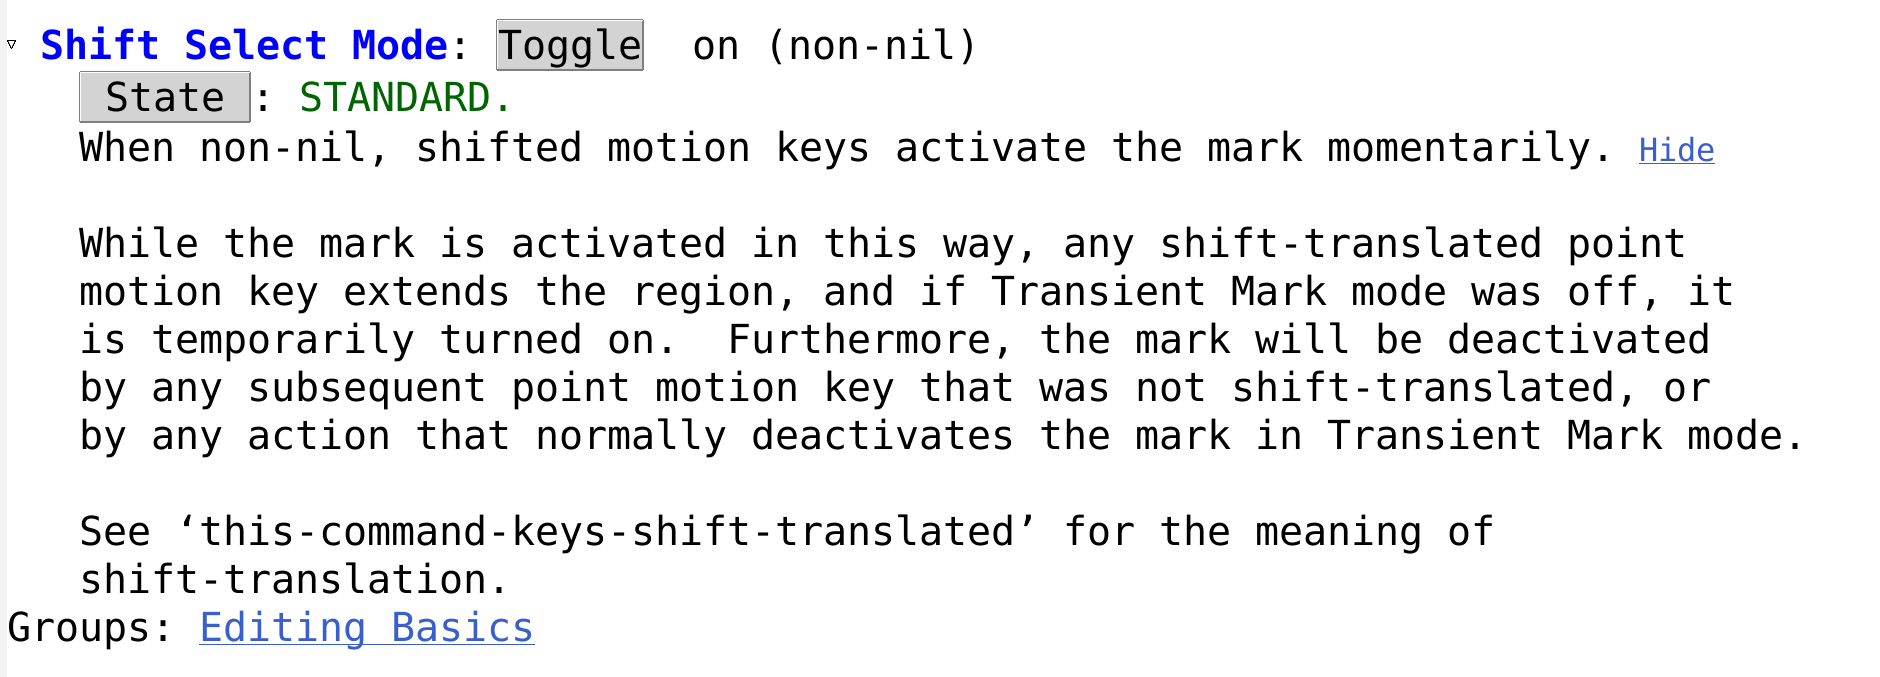
\includegraphics[width=0.8\textwidth]{custom}
  \caption{Custom user interface}
  \label{fig:custom}
\end{figure}
%

期望用户使用 Emacs Lisp 进行定制创造了很高的门槛。作为应对,Per Abrahamsen 在 1996 年贡献了两个名为 \texttt{Custom} 和 \texttt{Widget} 的库,使用户可以通过界面而不是通过 Emacs Lisp 来定制变量的值。 \texttt{Custom} 首次随 Emacs 20.1、Xemacs 20.1 和 XEmacs 19.15 一起发布(XEmacs 19.15 在 XEmacs 20.0 发布之后)。图 \ref{fig:custom} 显示了 \texttt{shift-select-mode} 的界面。

Custom 最初是为了定制 Gnus 新闻阅读器而创建的。随着其被整合到 Emacs 和 XEmacs 中, Custom 也获得了 Emacs Lisp 的编程接口。通过 \texttt{defvar} 原始方式进行的 \texttt{shift-select-mode} 的声明如下:
%
\begin{verbatim}
    (defvar shift-select-mode t
      "When non-nil, shifted motion keys activate the mark momentarily.
       ...")
\end{verbatim}
%
\texttt{Custom} 库提供了 \texttt{defcustom},它支持以下声明:
%
\begin{verbatim}
    (defcustom shift-select-mode t
      "When non-nil, shifted motion keys activate the mark momentarily.
       ..."
      :type 'boolean
      :group 'editing-basics)
\end{verbatim}
%
这个声明启用了用于定制 \texttt{shift-select-mode} 的界面。作为布尔值的 \texttt{:type} 声明将 \texttt{Custom} 显示为一个 \texttt{Toggle} 按钮。Emacs Lisp 程序员可以进一步将多个 \texttt{defcustom} 变量组合为 group 来创建层次结构, \texttt{Custom} 也会将它转换为导航 API。\texttt{:type} 声明可以简洁地描述复杂的结构,如下所示:

\begin{verbatim}
    (defcustom cc-other-file-alist
      '(("\\.cc\\'"  (".hh" ".h")) ...)
      "Alist of extensions to find given the current file's extension.
    ..."
      :type '(repeat (list regexp (choice (repeat string) function))))
\end{verbatim}

根据这个 \texttt{:type} 声明, Custom 将生成一个适当的界面来操作该值,它是一个元素列表,每个元素是一个正则表达式和一个字符串列表或函数组成的序对。这个 \texttt{:type} 声明还可以起到文档的作用。 Custom 现在在 Emacs Lisp 代码中被广泛使用,并且将编程语言和界面紧密联系在一起。

\subsection{Unicode}
\label{sec:unicode}

随着 Unicode~\cite{Unicode6} 的普遍采用,Emacs 和 XEmacs 都支持这一标准。Emacs 21.1 通过将其作为另一个“国家”(national)字符集添加到系统中,增加了对 \texttt{utf-8} 编码系统的支持。这意味着来自 \texttt{utf-8} 文件的“é”与来自 \texttt{latin-9} 文件的“é”被认为是不同的字符。这种区别在之前就已经存在,例如在 \texttt{latin-1} 和 \texttt{latin-9}(以及许多其他字符集)之间,但在过渡到 utf-8 期间许多的用户同时使用了两种编码系统,从而接触到这个问题。因为这个原因,2001 年,Emacs 22.1 引入了一种有限的字符集统一形式。XEmacs 也在 2001 年的 21.4 版本做了同样的改进。

随着 Unicode 成为通用的文本表示形式并取代了许多早期的编码方式,Emacs 和 XEmacs 都开始努力使用 Unicode 替代内部的 MULE 表示。这一变化出现在 Emacs 23(2007 年)和 XEmacs 21.5(从大约 2010 年开始的一个独立分支)。因此,无论是在 Emacs 还是 XEmacs 中,字符的整数表示现在是其 Unicode 标量值。

%% FIXME: We should talk about string representations and
%% unibyte-vs-multibyte issues (for example, whether "\351" should be a string
%% containing the *character* #o351 (that is, "é") or the string containing the
%% *byte* #o351.

\subsection{Bignums}

令人惊讶的是,作为一种 Lisp 语言,Emacs Lisp 多年来都没有对任意大的整数(bignum)提供支持。整数范围受限于底层机器的字长,随着时间的推移,表示方式的改变也影响了 Emacs Lisp 中整数的确切可用范围(\ref{sec:data-representation} 节)。因此,处理超出 fixnum 范围的数字的各种函数不得不实现解决方案。值得注意的是 \texttt{file-attributes} 和 \texttt{current-time}。前者可以使用两个 fixnum 组成的序对表示 inode 号、设备号、用户 ID 和组 ID,并可以使用浮点数表示文件大小。后者返回一个数字列表来编码时间。整数范围有限还引发了另一个问题,即它限制了可以编辑的文件的最大大小。

此外,Emacs Lisp 在文本编辑之外的应用中越来越多,也必须实现解决方案。Calc 是一个高级计算器和计算机代数工具,自 2001 年起随 Emacs 发行,由于 Emacs Lisp 不支持 bignum 而不得不在 Lisp 中实现大数算术。

Jerry James 在 2004 年的 XEmacs 21.5.18 版本中使用 GMP 库~\cite{GMP}添加了大整数支持。在 Emacs 中,Gerd Möllmann 于 2001 年 10 月左右开始通过 GMP 添加对 bignum 的支持,但从未完成。直到 2018 年 8 月,Tom Tromey 在 Paul Eggert 和其他几位开发人员的帮助下,最终再次使用 GMP 将 bignum 支持添加到了 Emacs 中。

XEmacs 中对 bignum 的支持包括任意精度的整数、有理数和浮点数,这在构建时是可选的。因此,虽然它相当完整,但 XEmacs 的 Emacs Lisp 程序仍然不能依赖于 bignum 支持。因此,\texttt{file-attributes}、 \texttt{current-time} 和 Calc 仍未利用 bignum。

相比之下,Emacs 目前只支持任意精度的整数,但该功能通过在 Emacs 中捆绑 \texttt{mini-gmp} 库来无条件提供,以供在未安装 GMP 的系统上使用。不支持有理数和任意精度浮点数只是因为对这些功能缺乏兴趣。为了简化程序员的系统,支持被设置为无条件的:代码不需要为没有可用的 bignum 时保留替代的代码路径。因此, \texttt{file-attributes} 和 Calc 已被修改以使用本地 bignum。

有趣的是,在 Emacs 中,bignum 一直被视为可取的,但从未被视为足够重要,以克服需要 GMP 或其他多精度库的麻烦。改变权衡的决定性因素可能是到了 Emacs 25 时,大多数 Emacs 版本都链接了 GNUtls 库,该库包含 GMP 以进行加密操作(HTTPS 支持需要 GNUtls)。

引入 bignum 对 Emacs Lisp 提出了一些设计问题,因为以前整数始终是非封装的(unboxed)。这意味着快速的 \texttt{eq} 操作在浮点数上的行为与 \texttt{eql} 不同。因此,某些 Emacs Lisp 代码假设如果两个整数表示相同的数字,\texttt{eq} 操作将返回 true。bignum 是在堆上分配的,所以对于两个 bignum 来说,这个假设不一定成立。在 XEmacs 中,如果情况是这样,\texttt{eq} 操作可能会返回 nil,而这似乎并没有引起严重的问题。这个问题经过长时间的讨论也没有达成一致意见,Emacs 的维护者们采用了 XEmacs 的设计,因为让 \texttt{eq} 操作的行为像 \texttt{eql} 操作被认为成本太高,而且这是一个可以在以后轻松更改的决策,没有引入任何重大 bug 的风险,而反过来则不成立。

%% ** Major Differences Between 19.11 and 19.12
%% ============================================


%% The new function `type-of' returns a symbol describing the type of a
%% Lisp object (`integer', `string', `symbol', etc.)

%% Symbols beginning with a colon (called "keywords") are treated
%% specially in that they are automatically made self-evaluating when
%% they are interned into `obarray'.  The new function `keywordp' returns
%% whether a symbol begins with a colon.

%% `get', `put', and `remprop' have been generalized to allow you to set
%% and retrieve properties on many different kinds of objects: symbols,
%% strings, faces, glyphs, and extents (for extents, however, this is not
%% yet implemented).  They are joined by a new function `object-plist'
%% that returns all of the properties that have been set on an object.

%% New functions `plists-eq' and `plists-equal' are provided for
%% comparing property lists (a property list is an alternating list
%% of keys and values).

%% The Common Lisp functions `caar', `cadr', `cdar', `cddr', `caaar', etc.
%% (up to four a's and/or d's), `first', `second', `third', etc. (up to
%% `tenth'), `last', `rest', and `endp' have been added, for more
%% convenient manipulation of lists.

%% New function `mapvector' maps over a sequence and returns a vector
%% of the results, analogous to `mapcar'.

%% New functions `rassoc', `remassoc', `remassq', `remrassoc', and
%% `remrassq' are provided for working with alists.

%% New functions `defvaralias', `variable-alias' and `indirect-variable'
%% are provided for creating variable aliases.

%% New macro `push' destructively adds an element to the beginning of a
%% list.  New macro `pop' destructively removes and returns the first
%% element of a list.

%% How did XEmacs bootstrap?
%% Strings with text-properties? No.

\subsection{Terminal-Local and Frame-Local Variables, Specifiers}

在 1995 年,Emacs 19.29 添加了同时在多个不同的 X11 服务器上拥有窗口的功能。XEmacs 也有类似的演进。这导致了一项要求,即显示(display)的某些方面应该局限于一个窗口或一个输出设备。Emacs 将 GUI 窗口称为 \emph{frame},与 buffer 类似,Emacs 会维护对当前 frame(\emph{current frame})的引用,该引用确定了 GUI 操作的隐式目标。XEmacs 也通过显示上下文(display context)维护设备(\emph{device}),以区分不同的 TTY 和不同的 X11 服务器。

由于 buffer-local 变量已经允许根据上下文设置不同的值,Emacs 进一步加强了这种类比,引入了 \emph{terminal-local} 变量的概念。 terminal-local 变量是根据当前 frame 所属的 X11 服务器(终端)而具有不同值的变量。terminal-local 变量的数量很少,而且在 C 代码中预定义;它们主要在内部使用,用于跟踪键盘状态等事情;Emacs Lisp 程序无法创建其他 terminal-local 变量。

XEmacs 选择了一条不同的路径:从 1995 年开始,Ben Wing(在 Chuck Thompson 的原型基础上)实现了 \emph{specifier},这是一种管理依赖于广义 \emph{display context} 的属性的对象~\cite{XEmacsLispRef1998}。第一个原型实现与 XEmacs 19.12 一起发布。specifier 的值(它的实例)取决于其 \texttt{locale} ,可以是 buffer、window、frame、设备或 MULE 字符集,或者这些对象的某些属性。

Emacs 20 在 1998 年增加了将变量设置为 frame-local 值的功能。与 terminal-local 变量相反,任何变量都可以被设置为 frame-local 变量,此外,一个变量可以同时既是 frame-local 的又是 buffer-local 的。

在 2008 年,在开发 Emacs 23.1 期间,开发者发现并修复了几个在 let 绑定、buffer-local 变量和 frame-local 变量之间的边界情况交互中的一些错误(例如,在进入 let 绑定和离开之间将变量设置为 buffer-local 变量),并在随后决定变量不应同时既是 buffer-local 的又是 frame-local 的。

在解决这些错误的过程中,开发者明显发现 buffer-local 变量和 frame-local 变量的实现过于复杂,因此在 2010 年对实现进行了改进,以使代码中的不同可能状态更加明确。也就是在这个时候开发者决定逐步弃用 frame-local 变量。至于 buffer-local 变量,它们在 Emacs Lisp 中被广泛使用,而且用显式访问 buffer 对象的字段或属性替换它们会使 Emacs Lisp 代码变得复杂。相比之下,frame-local 变量并没有被广泛使用,而且可以很容易地通过传统的访问器访问 frame 属性来替代,因此很难在实现中证明其额外复杂性的合理性。因此,在 2012 年发布的 Emacs 24.1 中,不再允许对 frame-local 变量进行 let 绑定,在 2018 年发布的 Emacs 26.1 中,frame-local 变量已被完全移除。

\section{Post-XEmacs Period}           % 2007-now ?
\label{sec:post-xemacs}

在 1991 年到 2001 年期间,与 XEmacs 相比,Emacs 的改进速度相对较慢。但从 2001 年开始,Emacs 的步伐再次加快。在 2008 年,Richard Stallman 再次辞去 Emacs 的维护者职务,新的维护者们更热衷于推动 Emacs Lisp 的发展,而 XEmacs 在 2010 年左右开始失去了动力。

%% Sadly, many improvements in XEmacs have never been
%% incorporated back into Emacs.

本节讨论了 2010 年之后 Emacs Lisp 设计中一些显著的进展,而这些进展在 XEmacs 中迄今为止尚未出现。

\subsection{Lexical Scoping}
\label{sec:lexical-scoping}

当 Richard Stallman 开始开发 Emacs Lisp 时,词法作用域在 Lisp 家族中(包括 Common Lisp 和 Scheme)已成为确立的标准。自然,将词法作用域添加到 Emacs Lisp 中的问题已经被提出了很多次。

第一个实现出现得相当早,以 \texttt{lexical-let} 宏的形式出现,该宏是 Dave Gillespie 在 1993 年引入的新的 \texttt{cl.el} 的一部分。 \texttt{lexical-let} 宏执行了一种局部的闭包转换(closure-conversion)。虽然这个宏在许多包中被使用,但从来没有被认为是一个好的提供词法作用域的解决方案。这个有些冗长的名称可能是一个因素。此外,宏生成的代码比等效的动态作用域代码效率低,并且更难调试,因为基于回溯的调试器会显示宏展开的讨厌细节(gory details)而不是对应的源代码。因此,\texttt{lexical-let} 只在那些词法作用域真正有益的特定情况下使用。

动态作用域在实践中主要有两个缺点:

\begin{itemize}
\item \textit{缺少闭包}。一些包通过使用类似 \verb|`(lambda (x) (+ x ',y))| 的方式动态构建 lambda 表达式绕过了缺乏闭包的问题,但是这种方法存在各种问题,比如在闭包中的宏展开太晚,它的代码无法被字节码编译器看到。Emacs 23.1 引入了 curry 操作符 \texttt{apply-partially} 以覆盖类似的用例而不具有这些缺点。在所有这些情况下,程序员必须手动指定从环境中捕获哪些变量,在检测这方面的错误上,工具几乎没什么用。

\item \textit{变量名全局可见}。全局可见的变量名要求在选择本地变量名时更加小心。使用特定包前缀来命名所有全局变量的约定很好地避免了名称冲突:它不仅避免了全局变量之间的冲突,还避免了本地变量与全局变量之间的冲突,因为本地变量没有这样的前缀。唯一可能的冲突仅发生在不同函数的本地变量之间。在 Emacs Lisp 中,这些冲突往往只会在存在高阶函数的情况下发生。例如在以下代码中:
\begin{verbatim}
    (let ((lst (some-list)))
      (cl-every (lambda (x) (memq x lst)) elements))
\end{verbatim}
如果在调用其第一个参数之前 \texttt{cl-every} 恰好绑定了一个名为 \texttt{lst} 的本地变量,就会发生变量捕获。名字冲突在另一种特殊情况下也会成为问题,即字节码编译器:为了发出关于使用未声明变量的警告,字节码编译器只是检查该变量是否已为 Emacs 所知,对于那些在调用栈中的函数(例如字节码编译器本身的函数)局部绑定的变量,该检查总是返回 true。因此,为了不干扰其他局部绑定,字节码编译器中的一些代码使用了较长的局部变量名称,使得代码变得更加丑陋。更糟糕的是,这些“解决方案”从来都不是真正完善的。
\end{itemize}
%%

对于希望在 Emacs Lisp 中实现词法作用域的唯一完全令人满意的解决方案是,所有绑定构造默认使用词法作用域,并提供一种简单的方式来让某些变量使用动态作用域,就像在 Common Lisp 中一样。但与此同时必须坚决保持与现有 Emacs Lisp 代码的兼容性,尽管可以容忍某些罕见情况下的有限破坏。

绝大多数现有的 Emacs Lisp 代码对使用的作用域类型并不关心,无论是动态作用域还是词法作用域,在几乎所有情况下都会得到相同的结果。早期的 Emacs Lisp 代码就是如此,随着字节码编译器开始警告对未声明变量的引用,这一点变得更加明显。关于未使用变量的警告可能会促使更多的 Emacs Lisp 代码保持不关心作用域类型。但无论如何,尽管存在上述情况,很明显大多数 Emacs Lisp 包在某个地方依赖于动态作用域。因此,虽然有希望能够将 Emacs Lisp 切换到使用词法作用域,但如何找到需要使用动态作用域的少数位置以避免过多破坏现有代码这一点仍然不清楚。

在 2001 年,Matthias Neubauer 实现了一种代码分析工具,该工具并不试图找出需要使用动态作用域的地方,而是试图找出那些在词法作用域下不会改变结果语义的绑定情况~\cite{Neubauer01}。这个工具可以被用来自动地将 Emacs Lisp 包转换为一个具有词法作用域的 Emacs Lisp 版本,同时保持语义不变。采用这种方法的计划是为最终将 Emacs Lisp 代码迁移到 Scheme 中提供便利,但整个项目过于庞大,无法实现。

在 2001 年末,Miles Bader 开始在一个称为 \emph{lexbind} 的 Emacs 分支上工作,以支持词法作用域,该分支最终在 Emacs 24.1 中被纳入。他采用的解决方案是使用两种语言:一个是带有动态作用域的 Emacs Lisp,用于向后兼容;另一个是具有类似 Common Lisp 的作用域规则的语言:默认为词法作用域,除了那些被声明为动态作用域的变量(实际上,这些都是全局变量)。每个文件都被标记以指示要使用的语言,默认为向后兼容模式。相应地,每个函数值都带有它所使用的语言的标记,因此使用动态作用域的函数可以无缝调用使用词法作用域的函数,反之亦然。这样,旧代码仍然可以像以前一样正常工作,而任何希望从词法作用域中受益的新代码只需在文件开头添加相应的 ``;; -*- lexical-binding:t -*-'' 注释。

这两种语言非常相似,以至于新的词法作用域变体只需要对现有解释器进行一些微小的更改。但是,为了在字节码编译器中支持这种新语言需要进行更多的修改,这导致这个分支的进展较慢。这个分支与主要的 Emacs 开发保持同步,但是对字节码编译器的修改从未完成。

%% https://lists.gnu.org/r/emacs-devel/2001-10/msg00560.html
最终,在 2010 年,Igor Kuzmin 在 Stefan Monnier 的指导下进行了一个暑期项目,在该项目中他尝试以不同的方式向字节码编译器添加词法作用域:他没有直接在单 pass 的字节码编译器代码中添加对词法作用域和闭包的支持(这需要对代码进行重大改动,并且由于需要在单 pass 中完成,使得代码变得更加复杂),而是实现了一个单独的 pass (它自身分为两个步骤)来执行传统的闭包转换。这种方法使闭包转换摆脱了单 pass 字节码编译器设计所施加的限制,使得实现变得更加容易,并且它还显著减少了字节码编译器中所需的改动量,从而降低了引入退化(regression)的风险。

两年后,Emacs 24.1 发布了,其中包含了基于 Miles Bader 的 \emph{lexbind} 分支和 Igor 的闭包转换的词法作用域支持。那时的主要关注点是:
\begin{itemize}
\item 最小化对现有代码的更改,以限制与现有 Emacs Lisp 包的不兼容性;
\item 确保现有代码的性能不受新特性的明显影响;
\item 提供可靠的对新词法作用域模式的支持,尽管不一定具有最佳性能。
\end{itemize}
%%

字节码的更改是作为词法作用域特性的一部分引入的,该特性于 2012 年在 Emacs 24.1 中出现,但实际上早在 2003 年左右就已经开发了:在引入词法作用域之前,基于堆栈的字节码只以最简单的方式使用堆栈,并且没有包含除 \texttt{pop/dup/exch} 之外的任何堆栈操作,为了更好地支持在堆栈上存储词法变量的词法作用域,开发者添加了几个字节码用于直接在堆栈中索引、修改堆栈槽和一次性丢弃多个堆栈元素。

除了与 \texttt{catch}、\texttt{condition-case} 和 \texttt{unwind-protect} 原语的交互之外,新的词法作用域模式的性能与动态作用域模式相比表现出了竞争力。这些原语的底层字节码与词法作用域不匹配,需要在运行时构建 Emacs Lisp 代码,以将词法上下文传递到这些构造的主体中。因此,在 Emacs 24.4 中引入了新的字节码,并修改了字节码编译器以能够利用它们。现在,使用词法作用域编译的代码通常预期比使用动态作用域编译的代码略快。

Emacs 24.1 引入词法绑定的过程非常顺利,对用户而言只造成了少数不向后兼容的改变,部分原因是 Emacs 自身的文件中很少使用词法绑定。将现有代码转换为使用新语言通常很容易(主要是添加几个变量声明,并借助字节码编译器的警告),但这并不是自动化的过程,有时可能需要进行较大的努力,特别是对于那些大量或创造性地使用动态作用域的包而言。如今,大多数新的包选择使用新的词法作用域语言,大约一半的维护良好的包已经进行了转换。然而,仍然有大量的代码使用旧的语言,这可能是因为它们仍然想要支持早于 Emacs 24.1 的 Emacs 版本,或者是因为转换需要的工作量。例如,截至 Emacs 26,只有三分之一的 Emacs 自身的 Lisp 代码已经转换为使用词法作用域。

\subsection{Eager Macro-Expansion} %Emacs~24.3?
\label{sec:eager-macro-expansion}

在 Emacs Lisp 中宏的展开时间从未被明确指定。直到 Emacs 24 版本,解释执行代码中的宏展开通常尽可能晚地进行,而对于字节编译的代码,宏展开总是在字节码编译期间进行,除了一些特殊情况,其中代码对字节码编译器是“隐藏的”。在字节码编译器中,宏展开也是“延迟”(lazily)进行的,即在编译的单次 pass 中动态地进行扩展。

为了在 Emacs 24 中实现单独的闭包转换阶段,这种行为必须进行更改,以便在实际的闭包转换和字节码编译之前使用新的 \texttt{macroexpand-all} 函数对代码进行独立的宏展开。这导致某些边缘情况下出现了一些可见的差异,之前在宏展开之前被优化消除的一些宏调用现在被展开了。在实际中这并没有引起任何严重的退化。

在 Emacs 24.3 中,对新的 \texttt{macroexpand-all} 函数的使用更加普遍,当加载非编译文件时会应用该函数。这意味着宏展开现在在加载文件时会立即进行,而不是在 Emacs 实际运行代码时惰性展开。这种激进(eager)宏展开有时会遇到依赖关系的问题(通常是在从未编译过的文件中),因此它会进行优雅的失败处理:如果在加载文件时的宏展开过程中发生错误,Emacs 会中止宏展开并继续处理非展开的代码,就像过去一样,尽管会适当地向用户通知问题所在。

Emacs 25.1 还根据 Common Lisp HyperSpec~\cite{HyperSpec} 的 3.2.3.1 节对这些宏展开阶段进行了微调(无论是加载文件时还是编译文件时),以改进展开为定义且使用这些定义的宏的处理方式。

\subsection{Pattern Matching}           %Released in Emacs~24.1
\label{sec:pcase}

在开发 \texttt{lexical-binding} 特性的过程中,Stefan Monnier 对用于遍历抽象语法树的代码形式感到越来越沮丧。相比于静态类型的函数式语言中使用的代数数据类型,这些代码中的 \texttt{car}、\texttt{cdr} 函数提供的信息太少了。

因此,他开始着手开发一种受这些语言启发的模式匹配构造。在开始这个项目之前,他搜索了现有的提供此类功能的库,发现了许多适用于 Common Lisp 和 Scheme 的库,但没有一个符合他的期望:要么生成的代码效率不够高,要么代码似乎难以移植到 Emacs Lisp,要么接受的模式集合过于有限且不易扩展。

于是,\texttt{pcase.el} 包诞生了,首次作为 Emacs 24.1 的一部分发布,并在提供对词法作用域支持的字节码编译器的部分中广泛使用。

除了提供类似于 Common Lisp 的 \texttt{case} 宏的超集 \texttt{pcase} 宏外,该包还提供了 \texttt{pcase-let} 宏,它使用相同的机制并支持相同的模式来解构对象,但它允许假设模式匹配成功,因此可以跳过所有测试,只保留提取数据的操作。

在 Emacs 24.1 发布后,Stefan Monnier 意识到了 Racket 的 match 构造~\cite{RacketReference2018},这个构造在他早先搜索现有的模式匹配宏时不知何故被忽略了,它的设计使得定义新模式变得容易。Racket 的 \texttt{match} 实现无法在 Emacs Lisp 中轻松重用,因为它过于依赖 Racket 对局部定义函数和尾调用的高效处理,但 \texttt{pcase.el} 得以改进以采用 Racket 的 \texttt{match} 设计的一部分。新版本出现在 Emacs 25.1 中,主要的创新点是引入了 \texttt{pcase-defmacro},可以使用模块化的方式定义新模式。
%% often using the new low-level pattern \texttt{app}.

\subsection{CL-Lib}          %Released in Emacs~24.3
\label{sec:cl-lib}

多年来,Emacs Lisp 的核心演变缓慢,而其他 Lisp 方言(主要是 Scheme 和 Common Lisp)的演进却在不断进行,这对 Emacs Lisp 增加各种语言扩展提出了压力。事实上,Emacs Lisp 可以近似地看作 Common Lisp 的子集,因此在 1986 年,Cesar Quiroz 已经编写了一个名为 \texttt{cl.el} 的包,该包通过宏提供了各种 Common Lisp 的功能。1988 年的 Emacs 18.51 版本是第一个内置 \texttt{cl.el} 的 Emacs 版本。在 5 年后的 Emacs 19.18 中,Dave Gillespie 贡献了一个新版本的 \texttt{cl.el},它更详细地模拟了 Common Lisp,并添加了一些扩展功能。

RMS 从来不希望 Emacs Lisp 逐渐演变为(morph into)Common Lisp,但他认识到提供这样的功能的价值,所以 \texttt{cl.el} 在 Emacs 中相对较早地被包含了进来,并成为最受欢迎的包之一,被大部分 Emacs Lisp 包所使用。然而,RMS 并不想强迫任何 Emacs 用户使用 \texttt{cl.el}。因此,他制定了一项政策来限制在 Emacs 中使用 \texttt{cl.el} 的范围:与 Emacs 捆绑在一起的 Emacs Lisp 包只能以一种在正常编辑会话中无需加载 \texttt{cl.el} 的方式使用 \texttt{cl.el}。具体来说,这意味着在 Emacs 中只能使用 \texttt{cl.el} 的宏和内联函数这些特性。

RMS 不希望使用 \texttt{cl.el} 并不想让 Emacs Lisp 变成 Common Lisp 的原因并不完全清楚,但以下因素似乎是其中的一部分动机:
\begin{enumerate}
\item 那个时候,Common Lisp 被认为是一门非常庞大的语言,因此要使 Emacs Lisp 真正成为一个合理完整的 Common Lisp 实现很可能需要付出相当大的努力。
\item Common Lisp 的某些设计方面可能会带来显著的开销,而 Emacs 本身已经被认为太庞大了(在那个八兆字节仍然是相当大的内存容量的年代,\texttt{vi} 的支持者们用贬低性的称谓(derogatory epithet)\emph{“eight megabytes and constantly swapping”}来嘲笑 Emacs 的内存占用情况)。因此,避免让 Emacs Lisp 的效率变得更糟糕是有充分理由的。
\item 许多 Common Lisp 设计的方面是由多数人而非共识决定的,这可以从 Common Lisp 和 Scheme 之间的分歧中看出。RMS 不喜欢 Common Lisp 设计中的几个方面,比如在像是 \texttt{mapcar} 的低级原语中使用关键字参数~\cite{RMS-keyword-args-are-clunky}。
\item 保持 Emacs Lisp 的简洁意味着用户可以参与其中的开发,而无需学习所有 Common Lisp 的知识。当讨论是否包含 Common Lisp 特性时,RMS 通常会指出其带来的成本,包括需要更多、更复杂的文档~\cite{RMS-cl-big-doc}。
\item \texttt{cl.el} 的实现具有相当的入侵性,会重新定义一些核心的 Emacs Lisp 函数。
\item 最后,将 Emacs Lisp 变成 Common Lisp 意味着失去了控制权,因为 Emacs 在很大程度上将受到 Common Lisp 发展的约束,必须遵守 Common Lisp 设计者在大多数方面的决策。
\end{enumerate}

多年来,前两点的重要性在一定程度上有所减弱。同时,\texttt{cl.el} 包的流行度以及 Emacs 贡献者不断要求更多 Common Lisp 特性的压力也减少了第四点的相关性。

XEmacs 在这方面采取了简单的方法,从 1996 年的 XEmacs 19.14 开始将 \texttt{cl.el} 加载到标准 XEmacs 映像中。Emacs 则选择了一条更长的道路,经过多年的筛选发现 \texttt{cl.el} 中的一些宏和函数足够清晰且受欢迎,以至于有理由将它们移植到 Emacs Lisp 中:


\begin{itemize}
\item 1997 年发布的 Emacs 20.1 版本移植了 \texttt{when} 和 \texttt{unless} 宏以及 \texttt{caar}、\texttt{cadr}、\texttt{cdar} 和 \texttt{cddr} 函数。
\item 2001 年,Emacs 的维护者 Gerd Möllmann 对 Common Lisp 有了更积极的看法。因此,Emacs 21.1 版本包括了散列表函数,这些函数经过了 C 语言的重新实现和扩展。它还采用了 Common Lisp 的关键字符号概念,以便更方便地支持 \texttt{cl.el} 以及其他使用这些符号的包。关键字符号是以冒号开头的符号;它们是自引用的字面量,表达式 \texttt{:foo} 的求值结果是 \texttt{:foo} 本身。这使得关键字符号在指定关键字参数时在记法上很方便。 此外还添加了宏 \texttt{dolist}、\texttt{dotimes}、\texttt{push} 和 \texttt{pop} 到 Emacs Lisp 中,尽管它们引入了一些困难:在 \texttt{cl.el} 中,这些宏包括了额外的功能,它们依赖于核心 Emacs Lisp 中不需要的 \texttt{cl.el} 部分,特别是 \texttt{block/return} 和广义变量。因此,添加到 Emacs Lisp 中的宏并没有真正取代 \texttt{cl.el} 中的宏;相反,当加载 \texttt{cl.el} 时,它会用自己的版本覆盖原始的宏。
\item 2007 年,Emacs 22.1 版本添加了 \texttt{delete-dups} 函数,它提供了 \texttt{cl.el} 中 \texttt{delete-duplicates} 的一个子集。
\item 2012 年,Emacs 24.1 版本添加了 \texttt{macroexpand-all} 和词法作用域,这使得 \texttt{cl.el} 中的 \texttt{lexical-let} 形式过时了。
\item 2013 年,Emacs 24.3 版本添加了编译器宏、\texttt{setf} 和广义变量。
\item 2018 年,Emacs 26.1 版本在 Emacs 20.1 中引入的 \texttt{cXXr} 函数的基础上,添加了剩余的 \texttt{cXXXr} 函数。对这些函数的抵制主要是出于代码风格的原因,因为它们往往导致难以阅读的代码。
\end{itemize}

这里的细节并不重要,而重要的是从 \texttt{cl.el} 到 Emacs Lisp 逐渐渗入了一系列功能,并且在许多情况下,这并不仅仅是将代码从 \texttt{cl.el} 移动过来,而是重新实现它,通常会有略微不同的语义。

在开发 Emacs 24.3 期间,更好地整合 \texttt{cl.el} 包的问题再次出现。主要的压力点是希望在与 Emacs 捆绑的包中使用 \texttt{cl.el} 函数 。RMS 仍然持反对态度,但这次找到了一个折中方案:用一个名为 \texttt{cl-lib.el} 的新包替换 \texttt{cl.el} 包,该包提供相同的功能,但所有的名称都使用 \texttt{cl-} 前缀。这样,\texttt{cl-lib.el} 包不会将 Emacs Lisp 变成 Common Lisp,而是在自己的命名空间下提供 Common Lisp 功能,使 Emacs Lisp 可以自由地按照自己的方式发展~\cite{RMS-cl-real}。

\texttt{cl-lib} 的实现主要是为 \texttt{cl.el} 中的定义添加了 \texttt{cl-} 前缀,同时实现了一个新的 \texttt{cl.el},它只是一个非常薄的包装器,将 \texttt{cl-lib} 的定义重新导出为它们的旧名称。这个薄包装器非常简单,既不会增加太多维护成本,也不会影响性能。\texttt{cl.el} 的一些实现细节也经过重新调整,变得更加非侵入性。特别地,\texttt{cl.el} 曾经用自己的实现全面重新定义了 Emacs 的宏展开,其中包括对编译器宏、\texttt{lexical-let}、\texttt{flet} 和 \texttt{symbol-macrolet} 的支持。标准的宏展开代码经过调整,以便 \texttt{cl-lib.el} 可以更清晰地提供这些功能。

为了鼓励适配这个新的库,一个用于旧版 Emacs 和 XEmacs 的 \texttt{cl-lib.el} 的向前兼容版本与 Emacs 24.3 同时发布了。尽管使用 \texttt{cl-} 前缀可能会引起一些对这个新库的抵触,但从新包中使用 \texttt{cl-lib.el} 而不是 \texttt{cl.el} 的比例来看,这个改动令人惊讶地成功了。

如今,Emacs 中同时捆绑了 \texttt{cl-lib.el} 和 \texttt{cl.el},并提供支持,但 \texttt{cl.el} 不再被 Emacs 自身的 Lisp 代码使用,预计在 Emacs 27 中将被宣布为过时。但由于它在多年来非常受欢迎,因此在真正废弃它之前还需要很长时间。

\subsection{Generalized Variables} %Released in Emacs~24.3
\label{sec:generalized-variables}

为了方便过渡到 \texttt{cl-lib.el},一些在 \texttt{cl.el} 中经常使用的功能被直接移植到 Emacs Lisp 中。其中最显著的是对广义变量(\emph{generalized variables})的支持,也被称为 \emph{places}、\emph{generalized references} 或 \emph{lvalues}。广义变量是一种既可以作为表达式又可以作为可更新引用的形式。这个概念源自 Common Lisp,在 Emacs 的实现最初是 \texttt{cl.el} 的一部分。在 Common Lisp 和 Emacs 中,一些特殊形式接受广义变量作为操作数。例如,\texttt{(setf \id{PLACE} \id{VALUE})} 将广义变量视为引用并设置其值。

在 Common Lisp 中,宏可以调用 \texttt{get-setf-expansion} 将一个 \emph{place} 转换为包含五个元素的列表:
\begin{displaymath}
  (\id{VARS}~\id{VALS}~\id{STORE-VAR}~\id{STORE-FORM}
  ~\id{ACCESS-FORM})
\end{displaymath}
\id{VARS} 和 \id{VALS} 共同构成一个绑定列表,用于执行访问该 place 所需的计算,这些计算只应该被执行一次(出于性能或副作用的考虑);\id{ACCESS-FORM} 读取该 place 的当前值;\id{STORE-VAR} 和 \id{STORE-FORM} 指定如何\emph{set} 该 place (通过将 \id{STORE-VAR} 绑定到所需的值,然后执行 \id{STORE-FORM})。

例如,宏 \texttt{(push \id{EXP} \id{PLACE})} 将 \id{EXP} 添加到存储在 \id{PLACE} 中的列表的头部,可以定义为展开为:
%
\begin{displaymath}
  \MAlign{
    \texttt{(let ((v \id{EXP}))} \\
    \;\;\;\texttt{(setf \id{PLACE} (cons v \id{PLACE})))}}
\end{displaymath}
%
但是这样会重复使用 \id{PLACE},它可能执行耗时的操作并具有副作用。因此,该宏使用 \texttt{get-setf-expansion} 以展开成以下形式的代码:

\begin{displaymath}
  \MAlign{
    \texttt{(let ((v \id{EXP}))} \\
    \;\;\;\MAlign{
      \texttt{(let* (\id{VARS} = \id{VALS})} \\
      \;\;\;\MAlign{
        \texttt{(let ((\id{STORE-VAR} (cons v \id{ACCESS-FORM})))} \\
        \;\;\;\id{STORE-FORM}))}}}
\end{displaymath}

这种方式强加了一个相当刻板的结构,虽然足够通用以适应大多数需求,但会带来负担并导致繁琐的代码和大量的冗余,不论是在实现 place 的过程中还是在接受 place 作为参数的宏的实现中。

原始的 \texttt{cl.el} 代码遵循了这种 Common Lisp 的设计。但是在实现 Emacs Lisp 中的 \texttt{setf} 和相关功能时采用了全新的实现概念。采用新实现的原因有以下几点:

\begin{itemize}
\item \texttt{cl-lib} 的实现者 Stefan Monnier 发现现有的代码很难理解,可以说是 Stefan 本人的一种“NIH 综合症”(not-invented-here syndrome,指一种心理现象,即对外部或已有的解决方案持怀疑态度,更倾向于自行开发或重新实现相似的解决方案,就是造轮子综合征)。
\item 之前的代码使用了 \texttt{cl.el} 中的内部辅助函数,而维护者们不想将其移植到核心的 Emacs Lisp 中,因此仍然需要进行一些重大调整。
\item Stefan Monnier 认为这部分 Common Lisp 的设计很丑陋。
\end{itemize}

%% For example, if we want to define a place
%% of the form $\texttt{(if~\textsl{TEST}~\textsl{PLACE1}~\textsl{PLACE2})}$
%% the above \texttt{push} will inevitably end up with one of two
%% possibilities:
%% \begin{itemize}
%% \item Check twice whether \textsl{TEST} was nil or not: once within
%%   \textsl{ACCESS-FORM} and once within \textsl{STORE-FORM}.
%% \item Do the check once within \textsl{VALS} to return a pair of an ``access
%%   function'' and a ``store function'' which are then called via
%%   \texttt{funcall} within \textsl{ACCESS-FORM} and \textsl{STORE-FORM}.
%% \end{itemize}
%%

因此,新的实现采用了不同的设计:与 Common Lisp 的五元组相比,新的函数 \texttt{gv-get-place-function} 将一个 \emph{place} 转换为一个单独的高阶函数。这个高阶函数以一个接受两个参数(\textsl{ACCESS-FORM} 和 \textsl{STORE-FUNCTION})的函数作为其唯一参数,该函数应返回我们要在该 place 上执行的代码。例如,\texttt{push} 宏可以这样实现:

\begin{verbatim}
    (defmacro push (EXP PLACE)
      `(let ((x ,EXP))
         ,(funcall (gv-get-place-function PLACE)
                   (lambda (ACCESS-FORM STORE-FUNCTION)
                     (funcall STORE-FUNCTION `(cons x ,ACCESS-FORM))))))
\end{verbatim}
%% and this can be streamlined a bit with the use of the macro
%% \texttt{gv-letplace} which lets us write the above as:
%% \begin{verbatim}
%%     (defmacro push (EXP PLACE)
%%       `(let ((x ,EXP))
%%          ,(gv-letplace (ACCESS-FORM STORE-FUNCTION) PLACE
%%             (funcall STORE-FUNCTION `(cons x ,ACCESS-FORM)))))
%% \end{verbatim}

这种设计一般会带来更清晰、更简单的代码,并且我们可以很容易地为大多数 Common Lisp 原语提供向后兼容的包装函数。

将一个 Common Lisp 风格的 place 表达式转换为相应的高阶函数是很容易的。然而,反过来却不成立,因此这种设计不兼容 Common Lisp 和 \texttt{cl.el} 的 \texttt{get-setf-expansion},后者必须产生上述五个值。当然,破坏与 \texttt{get-setf-expansion} 的兼容性是一个不足之处,但实际上这个函数几乎从未在 \texttt{cl.el} 之外被使用过,所以很少有包受到这种不兼容性的影响。

\subsection{Object-Oriented Programming} %Emacs~25.1
\label{sec:oop}

虽然 \texttt{cl.el} 在早期就提供了与 Common Lisp 的 \texttt{defstruct} 的兼容性(\ref{sec:structures} 节),包括定义新的结构作为其他结构的扩展/子类型,从而提供了有限的继承形式,但在 Emacs 中,对面向对象编程的实际支持,例如方法调度,在历史上一直有限。

向这个方向迈出的第一步是由 Eric Ludlam 在 1995 年底至 1996 年初开发的 EIEIO。它的正式名称“Enhanced Implementation of Emacs Interpreted Objects”暗示了早期存在某个“Emacs Interpreted Objects”包,但实际上首字母缩写在选择其扩展名称之前就已存在,因为这与童谣的滑稽引用有关\footnote{译注,E~I~E~I~O,出自经典英语儿歌 \emph{Old MacDonald Had a Farm}}。EIEIO 最初是一个尝试在 Emacs 中使用对象系统的实验,最初遵循类似于 C++ 的模型,但很快转向了受 CLOS 启发的模型。

\subsubsection{CLOS}

EIEIO 是 CLOS(Common Lisp Object System)的一个子集实现~\cite{DeMichielGabriel1987}。CLOS 是一个略显不寻常的对象系统,其中方法不附加到对象或类上;相反,它提供了通用函数(\emph{generic function})的概念,这些函数由一组方法实现,每个方法通过为其参数添加一个特化器(\emph{specializer})来指示其何时可用,通常是一个表示该方法仅适用于某类型参数的类型。这种基于类型的分派不仅限于第一个参数,还可以应用于任意数量的参数,这个特性被称为多分派(\emph{multiple-dispatch})。此外,当有多个方法可以应用时,程序员可以控制方法的组合(\emph{combine}),例如通过添加限定词(\emph{qualifier},如 \texttt{:after} 或 \texttt{:before})。除了通用函数,CLOS 还提供了 \texttt{defclass} 宏,用于通过列举其父类、字段和各种其他属性来定义新类型。

以下是一个 CLOS 代码的示例,它定义了一个新的 \texttt{point3d} 类作为现有 \texttt{point2d} 类的子类,并向通用函数 \texttt{point-distance} 添加了一个新的方法,但仅当两个参数都是 \texttt{point3d} 的子类型时才适用:
\begin{Verbatim}[samepage=true]
    (defclass point3d (point2d)
      (z :documentation "Third dimension"))

    (defmethod point-distance ((p1 point3d) (p2 point3d))
      (let ((distance2d (call-next-method))
            (distancez (- (slot-value p1 'z) (slot-value p2 'z))))
        (sqrt (+ (* distance2d distance2d)
                 (* distancez distancez)))))
\end{Verbatim}

\subsubsection{EIEIO}

就像 Emacs Lisp 一样,EIEIO 的发展主要是根据实际需求而不是为了自身而存在:最初的动机是尝试用于对象请求代理(object request broker,ORB,是一种中间件,充当对象之间的中介,协调请求和响应之间的通信),然后是 widget 工具包,后来切换到为 CEDET 包提供支持,CEDET 是一个提供类似 IDE 功能的包~\cite{Ludlam18}。EIEIO 包括对大多数 CLOS 的 \texttt{defclass} 的支持,以及对 \texttt{defmethod} 的子集的支持,但仅限于基于第一个参数的单分派方法。此外,它只能基于 \texttt{defclass} 对象的类型进行分派。它对方法组合的支持也不完整,只允许使用 \texttt{:before} 和 \texttt{:after} 方法,而不支持 \texttt{:around} 或任何用户定义的其他限定词。

在 2010 年与 CEDET 的大部分一起被集成到 Emacs 23.2 中之前,EIEIO 在大部分时间都作为 CEDET 包的一部分存在。在 Emacs 内部使用 EIEIO 的情况相对有限,部分原因是惯性,但也因为 EIEIO 遇到了与 \texttt{cl.el} 类似的问题,即它不是“命名空间清洁”的。

\subsubsection{CL-Generic}

在 2014 年底,Stefan Monnier 开始清理 EIEIO,以便能够在 Emacs 的更多部分中使用它。主要意图是像 \texttt{cl-lib} 一样添加一个 \texttt{cl-} 前缀(而不是 \texttt{eieio-} 前缀,被认为太冗长而不太受欢迎),同时改进 \texttt{defmethod} 以支持 \texttt{:around} 方法和针对除了使用 \texttt{defclass} 定义的类型之外的其他类型的分派。但很快就显而易见的是,方法分派的实现需要进行彻底的改进:与典型的 CLOS 实现的前期构建组合方法并记住结果不同,EIEIO 的方法分派和 \texttt{call-next-method} 在运行时动态执行所有工作,依赖全局变量来保留状态。这种方法不仅不稳定和低效,而且难以扩展来使用 \texttt{:around} 方法。

因此,与其改进 EIEIO 的 \texttt{defmethod},不如在新的 \texttt{cl-generic.el} 包中实现完全新的 CLOS 的 \texttt{defmethod} 版本,它在 Emacs 25.1 中出现。最直接的缺点是在此过程中忘记了清理 EIEIO 的其他部分(其中实现了 \texttt{defclass} 对象)。该实现并未过度优化,但已经比 EIEIO 中的先前版本快几倍。该包提供了与 CLOS 的 \texttt{defmethod} 基本相同的功能集,但存在一些重要的区别:

\begin{enumerate}
\item 方法组合无法像 CLOS 那样针对每个方法进行指定,而是只能通过向 \texttt{cl-generic-combine-methods} 添加适当的方法来全局添加新的方法组合。这个实现非常简单,但基本上无法使用,正如事实所证明的,在目前没有人使用这个功能,甚至在内部也没有人使用。
\item 支持的 specializer 并非硬编码。在 CLOS 中,specializer 可以是类型(表示当参数是该类型时该方法适用)或形如 \texttt{(eql \id{VAL})} 的形式,表示该方法仅适用于参数等于 \id{VAL} 的情况。Emacs Lisp 对此进行了扩展,可以通过 \emph{generalizer} 的概念以模块化的方式定义新的 specializer,这个概念受到了 Rhodes 等人的一篇论文的启发~\cite{Rhodes14}。这在内部被使用(用于定义所有标准的 specializer),以及在一些外部包中被使用,最值得注意的是在 EIEIO 中用于支持对 \texttt{defclass} 类型的分派。
\end{enumerate}

上述第一个区别的主要动机是因为 CLOS 对方法组合的支持看起来过于复杂:实现的成本无法与预期的功能用途进行合理的权衡,因此被一个更简单的机制所替代。

第二个区别是必需的,因为即使 \texttt{cl-generic.el} 不能依赖于 EIEIO,方法需要在 EIEIO 对象上进行调度。然而,还有其他的动机:能够定义新的 specialiazer 显然是可取的,而且它也使主要 specializer 的实现更加清晰,最重要的是,这似乎是一个解决起来很有趣的问题。

一些现有的 Emacs Lisp 函数似乎是使用这个机制将它们拆分为独立方法的好候选,但需要根据上下文信息(即当前状态)进行分派,而不仅仅是根据参数。因此,cl-generic.el 还为其 cl-defmethod 添加了对形式为 ``\&context (\id{EXP} \id{SPECIALIZER})'' 的伪参数的支持。这意味着当 \id{EXP} 求值为满足 \id{SPECIALIZER} 约束的值时,该方法是可用的。这用于只在特定上下文中适用的方法,例如特定的 major mode 或使用特定类型的 GUI 的 frame。

\subsubsection{Overall Support for Classes}

\texttt{cl-generic.el} 的实现伴随着对在线帮助系统的扩展,以便能够以类型为起点提供关于 Emacs Lisp 变量、函数、face 和其他类型的命名元素的信息。为了配合这一点,\texttt{cl-defstruct} 的实现得到了改进,以更好地保留有关类型层次结构的信息,以便可以使用在线帮助系统进行浏览。这最初是为了尝试将 EIEIO 的功能适应于 \texttt{cl-generic.el},以便可以交互地浏览 EIEIO 对象和方法,但现在更模块化并且与 Emacs 的其他在线帮助系统更好地集成在一起。

在 Emacs 26 中,Emacs Lisp 中的对象支持分为四个部分:由 \texttt{cl-lib.el} 提供的旧的 \texttt{cl-defstruct},它允许定义新的对象类型并支持单继承;由 EIEIO 提供的 \texttt{defclass},它提供类似的功能,还支持多重继承和一些其他的优点,但以创建对象和访问字段的速度较慢为代价;由 \texttt{cl-generic.el} 提供的 \texttt{cl-defmethod},它允许定义方法,并对 \texttt{cl-defstruct} 对象和 \texttt{defclass} 对象提供相同的支持;最后是 \texttt{defmethod},它已被重新实现为对新的 \texttt{cl-defmethod} 的包装(这个向后兼容的库已被弃用,并且比直接使用 \texttt{cl-defmethod} 效率略低,但仍比早期实现更高效,并且它完全使用了 \texttt{cl-defmethod} 的文档特性实现,因此不会引入任何性能或维护问题)。在可预见的将来,Emacs 可能会继续同时使用 \texttt{cl-defstruct} 和 \texttt{defclass}。

\subsection{Actual Objects}  %Emacs~26.1
\label{sec:actual-objects}

尽管 Emacs 25 的 \texttt{cl-generic.el} 为 Emacs Lisp 引入了面向对象编程的功能,但对象(无论是通过 \texttt{cl-lib} 的 \texttt{cl-defstruct} 还是 EIEIO 的 \texttt{defclass} 定义)仍然被表示为向量,因此无法可靠地与向量区分开来,例如进行漂亮的打印。

在 Emacs 26 中,通过引入 \texttt{make-record} 原语和相应的新对象类型(\ref{sec:structures} 节)解决了这个问题。记录(records)的实现方式与先前使用的向量完全相同,只是它们的标记(tag)表明应将它们视为记录而不是向量,并且按照约定,记录的第一个字段应该包含一个类型描述符,它可以是一个符号。

这种变化引入的主要复杂性是需要一种新的语法来打印和读取这些新对象,以及使用旧的基于向量的编码和使用新编码的对象的打印表示之间的不兼容性。

\subsection{Generators}
\label{sec:generators}

随着 Python 和 JavaScript 的迭代器和生成器的成功,一些 Emacs 用户觉得 Emacs Lisp 在抽象方面缺乏一些功能。因此,在 2015 年,Daniel Colascione 开发了 generator.el,并在 Emacs 25.1 中加入了该功能。它通过使用宏 \texttt{iter-lambda} 和 \texttt{iter-yield} 使编写生成器变得简单和方便。它的实现基于一种局部转换为延续传递风格(CPS),因此依赖于词法作用域的使用,以解决 Emacs Lisp 不直接提供类似 \texttt{call/cc} 的访问底层延续的问题。它只处理 Emacs Lisp 的一个相对较大的子集,因为在 Emacs Lisp 中一般无法定义类似 \texttt{unwind-protect}~\cite{HaynesFriedman1987}形式的 CPS 转换。

\subsection{Concurrency}
\label{sec:concurrency}

Emacs Lisp 是一种基本顺序的语言,并且在很大程度上依赖于对全局状态的副作用。然而,由于其在交互式程序中的使用,必然会希望引入并发性以尝试提高响应能力。并发性在很早之前就出现了:自从 Emacs 16.56 版本起,Emacs 就包含了对异步进程的支持,即执行独立程序并在 Emacs Lisp 执行引擎空闲等待下一次用户输入时,通过所谓的进程过滤器(\emph{process filter})处理其输出。

虽然这种非常有限的合作式并发性在 1994 年的 Lucid Emacs 19.9 和 1996 年的 Emacs 19.31 中通过添加对定时器的本地支持得到了一些改进(定时器先前以异步进程的形式在需要的时间向 Emacs 发送输出),但它一直是 Emacs 大部分生命周期中唯一可用的并发形式。

由于现有的 Emacs Lisp 代码广泛依赖共享状态,向 Emacs Lisp 添加真正的共享内存并发是有问题的。在某些情况下,共享状态不是一个问题,可以通过异步编程来模拟并发:当程序等待一个操作(比如外部程序)时,它会注册一个延续(continuation)回调并将控制权返回给主事件循环。然而,许多 Emacs Lisp 包会阻塞,因为通过回调来切片执行(slicing the execution)意味着实际上要以 CPS 编写代码,这在 Emacs Lisp 中没有得到很好的支持, CPS 与动态作用域交互很差,并且需要对现有代码进行重大改动。

因此,共享内存并发在很大程度上被认为不适用于 Emacs Lisp。即便如此,在 2008 年 11 月,Giuseppe Scrivano 发布了首个尝试向 Emacs Lisp 添加线程的 naive 版本。这个努力没有取得太大的进展,但它激发了 Tom Tromey 试试自己的运气。在 2010 年,他开始致力于向 Emacs 添加共享内存协作并发原语,比如 \texttt{make-thread}。与基于全局状态以提高速度的动态作用域实现的交互需要尝试各种方法。正确处理 buffer-local 绑定和 frame-local 绑定而无需进行完全重写是非常困难的,大多数方法都仅仅因为难以将它们与不断发展的 Emacs 代码库保持同步而被放弃。

最终,一种可行的方法在 2018 年作为 Emacs 26.1 的一部分发布了。上下文切换仍然只发生在几个已知的 Emacs Lisp 空闲点(或通过显式调用 \texttt{thread-yield})。当前实现中,上下文切换的时间与当前堆栈深度成正比,因为需要保存和删除旧线程的动态绑定,然后需要恢复新线程的动态绑定。早期的实现方法尝试通过增加全局变量查找的开销来避免这种昂贵的上下文切换方式,但这需要对现有代码进行更广泛和精细的更改。因此,尽管这种方法可能在未来被重新考虑,但当前的实现更倾向于采用更简单和更安全的方法。

主要维护人员之间对于包含这种共享状态并发形式的讨论非常激烈。他们都同意 Emacs Lisp 需要发展并发和并行性,以利用日益增多的 CPU 核心数量,特别是因为单核性能不再显著提高。但他们也达成共识,共享内存对于当前的 Emacs Lisp 环境来说非常不适合。最终只有 Tom Tromey 的补丁被接受,这是因为它不具有侵入性,并且有一种认识到有必要做些什么的感觉存在。

这仍然是一个相当实验性的功能,在出现两年后其使用似乎仍然局限于一些实验性补丁,例如 Gnus MUA 等少数几个包。可以说到目前为止,主要的结果是暴露了一些包中异步处理方面的潜在错误。

多年来,其他关于并发性和并行性的方法已经以 Emacs Lisp 包的形式开发出来,最显著的是 \texttt{async.el} 包~\cite{WiegleyAsync2019},它于 2012 年开发,可以在单独的 Emacs 子进程中并行运行 Emacs Lisp 代码。它的适用性受到限制,因为 buffer 内容需要在两个进程之间显式地按需发送,从而导致并行非常粗粒度。此外,不能保证子进程的配置与主进程一致 —— 在某些情况下,子进程甚至可能是 Emacs 的另一个版本。尽管如此,一些第三方包有限地使用了 \texttt{async.el}。

\subsection{Inline Functions}
\label{sec:inline-functions}

在 Emacs Lisp 中,函数调用是相当昂贵的,并且它们的语义涉及在全局命名空间中查找当前的定义,因此函数内联在性能和语义上都很重要。

因此,在开发 Emacs 19 的新字节码编译器期间添加了一个新的 \texttt{defsubst} 宏,它的工作方式类似于 \texttt{defun},但是会对函数进行标注,告诉字节码编译器尽可能内联它。这种内联化相当 naive,但适用于编译和非编译函数(通过将函数体内联到源代码或内联到调用者的字节码中)。

Dave Gillespie 在 1993 年引入的新包 \texttt{cl.el} 中,通过 \texttt{defsubst*} 宏引入了一种新的内联方式。从外部来看它与 \texttt{defsubst} 几乎相同,只是包含了对关键字参数等 Common Lisp 扩展的支持,但它的实现通过替换实际参数来生成更高效的代码(并不完全保持 Emacs Lisp 函数调用的通常语义)。

在 Emacs Lisp 中实现可内联的函数的第三种方式是将其定义为宏,尽管这带来一个缺点,即它不定义一个真正的函数。

2014 年末,Stefan Monnier 在将 \texttt{cl-lib} 库适应 EIEIO 和 \texttt{cl-defstruct} 对象的变化过程中对 \texttt{cl-typep} 的定义和编译器宏之间的冗余感到受挫。\texttt{cl-typep} 函数接受两个参数,并检测第一个参数是否是由第二个参数指定的类型的值。这个函数定义处理了类型参数只在运行时才知道的一般情况。编译器宏允许进行优化 —— 例如,它将 \texttt{(cl-typep x 'integer)} 转换为 \texttt{(integerp x)}。类型说明也可以采用 \texttt{(not \id{TYPE})} 的形式以表示“除 \id{TYPE} 之外的任何类型”、\texttt{(eql \id{VAL})} 表示包含特定值的类型、\texttt{(satisfies \id{PRED})} 表示给定谓词返回 true 的值的类型。

因此,Stefan Monnier 开发了新的宏 \texttt{define-inline},并在 Emacs 25.1 中加入了这个功能。它允许程序员使用单个表达式定义一个普通函数和相应的优化编译器宏。图 \ref{fig:define-inline} 展示了当前版本使用 \texttt{define-inline} 的 \texttt{cl-typep} 的骨架:它通过从函数体中删除 \texttt{inline-} 前缀来解释函数定义,同时定义编译器宏。前者在运行时执行 \texttt{pcase} 分派,后者在编译时执行。这样,如果 \texttt{type} 静态已知,则内联相应的分支;如果 \texttt{type} 静态未知,那么 \texttt{inline-const-val} 会检测到该问题,并完全放弃内联。目前,在 Emacs 发行版中有将近 50 个函数使用 \texttt{define-inline} 进行定义。

\begin{figure}
\begin{verbatim}
    (define-inline cl-typep (val type)
      (inline-letevals (val)
        (pcase (inline-const-val type)
          (`(not ,ty)         (inline-quote (not (cl-typep ,val ',ty))))
          (`(eql ,v)          (inline-quote (eql ,val ',v)))
          (`(satisfies ,pred) (inline-quote (funcall #',pred ,val)))
          ((and (pred symbolp) ty (guard (get ty 'cl-deftype-satisfies)))
           (inline-quote (funcall #',(get ty 'cl-deftype-satisfies) ,val)))
          ...
          (ty (error "Bad type spec: %s" ty)))))
\end{verbatim}
  \caption{Example use of \texttt{define-inline}}
  \label{fig:define-inline}
\end{figure}

%% Daniel Colascione: Do you want to mention how Emacs Lisp is _defined_ to
%% expand compiler macros, which, AIUI, distinguishes it from other lisps?
%% Stefan: I don't think it's defined to do that (after all, it happens only
%% in `macroexpand-all` but not in `macroexpand` so it does not happen
%% for interpreted code that's not eagerly macroexpanded).

\subsection{Module System}
\label{sec:module-system}

虽然 Emacs Lisp 从一开始就被设计为一种真正的编程语言,而不仅仅是一个小型的特定扩展语言,但它并没有为“大规模编程”而设计,这可以从缺乏模块或命名空间系统中看出。

然而,Emacs 的 Emacs Lisp 部分现在已经成为一个相当庞大的系统,为了避免名称冲突,Emacs Lisp 使用了一种简陋的命名空间系统。如 \ref{sec:lexical-scoping} 节所提到的。在这种系统中,代码遵循一种约定,属于包 \verb|<pkg>| 的全局函数和变量的标识符以 \verb|<pkg>-| 前缀开头(对于内部定义的标识符,则使用 \verb|<pkg>--| 前缀)。

有过很多通过提供对某种形式的命名空间的支持来纠正这种情况的尝试:

\begin{itemize}
\item 在 2011 年 5 月,Christopher Wellons 开发了 \texttt{fakespaces} 包,它允许定义私有变量和函数,并防止它们逸出到全局命名空间。非私有定义仍然依赖于通常的包前缀命名约定,以避免冲突。
\item 在 2012 年 10 月,Chris Barrett 开发了 \texttt{Namespaces} 包,它提供了一套广泛的新宏来定义命名空间,在这些命名空间中定义函数和变量,并从其他命名空间中使用它们。
\item 在 2013 年 3 月,Wilfred Hughes 开发了 \texttt{with-namespace} 宏的概念验证版本,该宏只是将指定的命名空间前缀添加到其主体中定义的所有元素中。
\item 与此同时,Yann Hodique 开发了概念验证的 \texttt{Codex} 包,该包试图提供类似于 Common Lisp 的 packages 功能,其中每个包都有自己的 \emph{obarray}。
\item 2014 年初,Artur Malabarba 开发了 \texttt{Names} 包,该包采用了 \texttt{with-namespace} 的方法,但在与代码操作工具(如 autoload 声明生成器)正确交互以及使源代码级调试器能够对单个声明进行插装方面做的更加彻底。
\item 2015 年,同样是 Artur Malabarba 开发了 \texttt{Nameless} 包,它采用了完全不同的方法:它不提供任何新的 Emacs Lisp 构造,而是专注于使 Emacs 在处理代码时\emph{隐藏用户}的包前缀。
\end{itemize}
%%

迄今为止,Emacs 尚未整合任何命名空间功能,其他软件包中也很少使用。最后一次关于这个主题的(激烈)讨论是在 2013 年,Nic Ferrier 在博客中发布了一篇文章~\cite{FerrierNamespaces}。在这一点上开发者没有形成共识,但除了惯性外,维持现状的主要论点之一是 Emacs Lisp 的简陋手工命名空间只是一个轻微的烦恼,而换来的是对于初学者和交叉引用的便利~\cite{namespace-discussion}:可以使用任何简单的文本搜索来查找任何全局函数或变量的定义和使用,包括全局文件系统搜索甚至网络搜索,而其他所有替代方案都引入了需要相对于上下文进行解释的名字,这迫使我们在浏览代码时依赖于能理解特定命名空间的 IDE。

%% FIXME: Should we talk about "package systems" in XEmacs / ELPA etc.?

%% \clearpage
\section{Conclusion}
\label{sec:conclusion}

% FIXME: check that nothing new is introduced
Emacs Lisp 最初主要是基于实际应用需求而发展的:RMS 对开发可编程编辑器感兴趣,而不是主要关注语言设计。他选择使用 Lisp 并不仅仅是出于即时的需求,而是受到当时他所处环境和经验的影响。因此,最初的 Emacs Lisp 尽可能简单,同时避免了 TECO 的缺点,并获得了 Maclisp 的大部分优势。

作为一种 Lisp 语言,Emacs Lisp 的核心语言自其最初创建以来并没有发生重大变化。其他许多语言中需要进行语言扩展的东西在 Emacs Lisp 中通常只是一个库。多年来,添加的内容主要是一些便利功能或者是由新的编辑器功能(尤其是图形界面)驱动的。Emacs 和 XEmacs 方言之间演变出的一些差异是由于对编程语言设计的不同观点所致,其中最明显的是对于不透明数据类型的使用。

随着 Gerd Möllmann 于 2000 年开始负责维护,并在 2008 年由 Stefan Monnier 和 Chong Yidong 接手维护工作,Emacs Lisp 的语言设计逐渐受到更多关注,并成为一个独立的目标。语言设计者的视角推动了一系列变化,例如引入了词法作用域、借鉴了 Common Lisp 的特性以及引入了 \texttt{pcase}。

Emacs Lisp 的核心语言基本保持原始形式不变,其实现方式也没有发生实质性的改变:任何重大的改动都会使大量的代码无效。此外,实现方式通常足以满足 Emacs 编辑器 30 多年来的需求。因此,Emacs Lisp 在可预见的未来不会消失:我们期待着报道它未来 30 年的演变。

% Many steps of \Elisp's evolution have been the result of efforts of single
% individuals, driven by a specific purpose, yet it has managed to keep an
% arguably sane and cohesive overall design, thanks on the one hand to
% a maintainership which was more interested in improving the text editor than
% the language and kept an eye on the longer term, and on the other to the
% willingness to break backward compatibility in specific cases, in order to
% gradually address problems encountered over time.

% \Elisp{}
% has steered a remarkably stable course of conservative development and
% gradual extension.  It has mostly grown by slowly incorporating popular
% features from other languages, both in the language itself and in its
% implementation.  But it has also come up with its own features, such as
% docstrings, buffer-local variables, the addition of text-properties
% to strings, and the custom library.

% The composability of the existing \Elisp{} packages relies on social
% mechanisms, and the organic growth of all the \Elisp{} packages has
% been able to maintain it for more than 30 years, keeping balkanization
% at bay to date.  Given the vast amount of changes Emacs users and
% developers have made to the system over the last decade alone, we are
% looking forward to the \Elisp{} of the next 30 years.

\begin{acks}
Emacs 和 Emacs Lisp 是许多人的贡献的结果。我们感谢他们所有人的贡献。尽管通过 Emacs 使用的各种版本控制系统来维护 Emacs 的修订历史的努力非常有帮助,我们也要感谢 Lars Brinkhoff 在 \url{https://github.com/larsbrinkhoff/emacs-history} 上的存档工作,它填补了 Emacs 早期发展的一些空白。此外,我们感谢 Joseph Arceneaux 在附录 \ref{appendix:arceneaux} 中的采访,以及 Richard Gabriel、Richard Stallman 和 Jamie Zawinski 耐心回答我们的问题。

这项工作得到了 \grantsponsor{NSERC}{Natural Sciences and Engineering Research Council of Canada}{http://nserc-crsng.gc.ca/} 的部分资助,资助号码为 N$^o$~\grantnum{NSERC}{298311/2012} 和 \grantnum{NSERC}{RGPIN-2018-06225}。本文中所表达的任何观点、发现、结论或建议均属于作者个人观点,不一定反映 NSERC 的观点。
\end{acks}

%% \clearpage                      %Looks cleaner, IMO  --Stef
\appendix

\section{Alternative Implementations}
\label{sec:alternative-implementations}

Emacs Lisp 的实现并不仅限于 Emacs 及其衍生版本。两个实现 —— Edwin 和 JEmacs —— 以在独立于 Emacs 实现的编辑器上运行 Emacs Lisp 代码而著名。此外,还有一个 Common Lisp 包模拟了 Emacs Lisp,并且 Guile Scheme 也提供了对 Emacs Lisp 语言的支持。这些实现的目标都是在替代环境中运行现有的 Emacs Lisp 代码,因此没有进行重大的语言更改。

\subsection{Edwin}

Edwin 是与 MIT Scheme 一起提供的编辑器~\cite{MITScheme2014}。它的用户界面基于 Emacs。Edwin 完全由 Scheme 实现,Scheme 是它的本地扩展语言。此外,Matthew Birkholz 在当时还实现了一个在 Scheme 中能够运行大规模 Emacs Lisp 包的 Emacs Lisp 解释器~\cite{Birkholz1993},其中包括 Gnus 新闻阅读器。

\subsection{Librep}

在 1993 年,John Harper 开始着手开发一种可嵌入的 Emacs Lisp 实现,称为 Librep,它最著名的应用是用作 Sawfish 窗口管理器的扩展语言。虽然 Librep 最初是一个与 Emacs Lisp 大部分兼容的 Lisp 方言,但它后来发展出了显著的差异,包括模块系统、词法作用域、尾递归消除和 first-class continuation。

\subsection{Elisp in Common Lisp}

在 1999 年,Sam Steingold 还将 Emacs Lisp 语言实现为一个 Common Lisp 包~\cite{Steingold99}。他的动机是希望将 Emacs 迁移为使用 Common Lisp 语言而不是 Emacs Lisp,并且希望在其他地方重用一些 Emacs Lisp 代码,尤其是来自 Emacs 的 Calendar 包。他的 \texttt{elisp.lisp} 包并不试图重新实现 Emacs 中用于操作 buffer 和其他相关对象的函数库,因此它专注于纯粹的 Emacs Lisp 语言;但它能够运行 Emacs Calendar 的非 UI 部分,该部分提供了复杂的函数来操作和转换多种历史日历之间的日期。

\subsection{JEmacs}

JEmacs~\cite{Bothner2001}是随 Kawa Scheme~\cite{KawaScheme}一起发布的一款编辑器。JEmacs 支持运行一些 Emacs Lisp 代码。它的实现(部分用 Java 编写,部分用 Scheme 编写)通过将 Emacs Lisp 代码转换为 Scheme 并运行转换结果来工作。

\subsection{Guile}

Guile Scheme~\cite{Guile2020}是 GNU 项目的通用扩展语言,并打算在某个时刻替代 Emacs 中的 Emacs Lisp~\cite{WhyNotTcl}。尽管目前还没有发生,但 Guile 提供了一个相当完整的 Emacs Lisp 实现来将 Emacs Lisp 程序转换为 Guile 的中间语言。它在 Guile-Emacs 系统中使用,这是对 Emacs 的一项正在进行中的修改,其中 Emacs Lisp 引擎由 Guile 提供。

\subsection{Emacs-Ejit}

在 2013 年,Nic Ferrier 实现了 Emacs-Ejit,一个使用 Emacs Lisp 编写的从 Emacs Lisp 编译到 Javascript 的编译器。它的设计目的是能够完全使用 Emacs Lisp 编写网站,使用 Elnode 包进行服务器端处理,并使用 Emacs-Ejit 在客户端中也使用 Emacs Lisp 编写代码。它并不真正指望在浏览器中运行任何 Emacs Lisp 包,因此其运行时库只提供了 Emacs Lisp 标准基本功能的一个小子集。

\section{Interview with Joseph Arceneaux}
\label{appendix:arceneaux}
\newenvironment{question}{\begin{quote}\itshape}{\end{quote}}

Joseph Arceneaux 是一名美国软件架构师。在 1990 年代初,Arceneaux 是 GNU Emacs 的维护者,先是在 FSF 工作,然后为 Lucid 公司工作。Lucid 公司希望将其用于 C++ 的 Energize IDE 基于 Emacs(\ref{sec:energize} 节)。在 Arceneaux 任职期间,Lucid 公司的商业利益与 Emacs 的原始作者 RMS 的利益发生冲突,最终导致 Lucid 创建了自己的 Emacs 分支 —— Lucid Emacs。

Arcenaux 很慷慨地同意在 2019 年 5 月 30 日接受 Michael Sperber 的采访。采访的目的是为本文提供背景资料,特别是 Emacs Lisp 在这次分歧中扮演的角色。

%
\begin{question}
能告诉我你是如何进入软件行业的吗,追溯到你如何涉足 Emacs
\end{question}
%

当我 15 或 16 岁的时候,我计划成为一名兽医。我很早就从高中毕业,因为我参加了一次考试,然后我上了一门计算机科学课程,对此产生了浓厚的兴趣。我进入了现在的路易斯安那大学(University of Louisiana),之后是西南路易斯安那大学(University of Southwest Louisiana),我有一位使用 Emacs 的芬兰教授,他说服我开始使用 Emacs。当我从研究生毕业的时候,我不仅仅在使用 Emacs,还为该项目贡献了代码,并对自由软件运动产生了兴趣。

毕业后,我去法国的 INRIA(国家计算机与自动化研究所)从事研究工作。作为一名研究人员,我有相当多的空闲时间用来进行 Emacs 的开发,并且我与 Richard Stallman 建立了很好的关系。我邀请他来 INRIA 做了几次讲座。这是 Stallman 第一次骑摩托车,当我带他去做讲座时,他快吓死了。

我们建立了这种专业关系,我继续为 Emacs 贡献代码,然后我的研究小组创办了一家初创公司。这是一个功能强大的 X 终端。那个时候 X Window 系统真正开始流行起来。我们有自己的硬件设计,我们的主要窗口专家将 X Window 系统移植到了我们的硬件上。我是系统方面的人,所以我写了 BIOS,并且我们采用了一种新的微内核操作系统,类似于 Mach,叫做 Chorus。随着我们公司的发展,公司内部变得越来越政治化,与此同时,Stallman,我们都称他为 RMS,因为那是他的登录名,邀请我加入自由软件基金会工作,我觉得这将是一个很好的职业发展机会,而且我非常享受为 Emacs 编写代码的乐趣。那时的 Emacs 主要由 Stallman 和像我这样的贡献者编写,主要结构由 Stallman 编写。我发现代码的结构大部分很容易理解,尤其是很容易进行扩展。偶尔我会提交一些东西,RMS 会拒绝,但大多数时候他都接受我的代码。他做过一些聪明的事情,这需要对计算机的工作原理有很深入的了解,但除了其中的两三个例子外,编写新代码真的很容易。

在自由软件基金会,我在麻省理工学院人工智能实验室度过了几年非常愉快的时光。我和 RMS 会偶尔就如何在 Emacs 中做某件事情进行争论。RMS 是一个非常聪明的人,他曾获得过麦克阿瑟天才奖。这期间发生过一些奇怪的事情,比如我接到一个电话,是来自挪威的人在询问混沌数学的事情。原来 RMS 是混沌数学的专家。所以当我们争论的时候,他赢了很多次。但我要说,他之所以能赢得争论,并不仅仅是因为他非常聪明。部分原因是因为他非常热情。我记得有一次我走下楼梯,他在我后面大声叫喊,然后我又追上楼梯追着他,他就捂住耳朵不听我的论点。所以他是一个有趣的人。不过,我也赢过一些争论。

其中一个重要的问题是窗口系统。正如我之前提到的,X Windows 变得非常流行。X Windows 开发组就在我们楼的二楼。在我看来,Emacs 需要成为一个完全集成了 X Windows 的系统。RMS 坚决反对这个想法。这并不是出于哲学上的原因,而是因为他认为有更重要的事情要做。一个已经与 X10 集成的 Emacs 版本效果还不错,但一旦转向 X11,它就无法工作了,而且没有人去进行移植(我记得这两个系统之间相当不兼容)。

有一些有趣的技术问题,例如:当时,在 buffer 中为每个字符关联特性的计算是不可取的。于是一个叫 Dan LaLiberte 的人提出了他所称的“intervals”系统。这个想法的基本是在 buffer 内容上建立一个影子结构。它的本质是:从这里到那里,我们使用的样式(face)是这个,从那里到另外那里是另一个样式。一个“样式”是一个包含颜色、字体、背景和其他特性的结构。我拿到了他写的东西并进行了原型设计,我完善了一些东西,并添加了一些其他功能,比如缓存,我们在 buffer 中的位置等等。当时我是 Emacs 的维护者,我在空闲时间里进行这个工作,并整合贡献。我开始将这视为 Emacs 的一个重要功能开发。RMS 仍然坚决反对这个想法。所以我不确定该怎么办,我和 FSF 的董事们进行了很多讨论。在某个会议上,我遇到了来自 Lucid 的法国人 Matthieu。我们相处得很好,部分原因可能是我会说法语。最终,Lucid 给我提供了一份合同,要求我将 Emacs 与 X11 集成,因为他们正在进行一个面向 C 和 C++ 的 IDE 项目,希望将 Emacs 作为主要界面。我和 RMS 在这个问题上发生了很大的争执,因为他不希望我这样做。我的论点是“嘿,这些人基本上会支付我的工资一段时间,我完成了这个任务,FSF 不需要付出任何代价。”董事会支持我的观点,但 RMS 不同意。所以我继续做那个项目,之后 RMS 一年左右不和我说话。此外,我在与 Lucid 签订合同后搬到了加利福尼亚。

我和 Lucid 的合同分为三个部分。第一部分是最具挑战性的,因为它必须在性能方面符合特定的规范。因此,如果我们拥有所有这些可视化注释信息,并且你对某个字符串进行搜索,要求是该搜索速度不应比没有可视化注释的任何 Emacs 版本慢。所以我通过了这个部分。我忘记了其他两个部分是什么,但在我的合同的第一阶段之后,Lucid 改变了他们希望前进的方向,并试图将我聘为全职员工。

\begin{question}
你还记得为什么 Lucid 改变了方向,或者为什么他们的需求发生了变化?
\end{question}
%
具体情况记不太清楚了。我觉得其中一部分是出于政治原因。但我不记得具体细节了。我只记得我们在选择方向上有争论。当时我重新与 RMS 取得联系,并开始将我的代码提交到 Emacs 的主要代码库中。RMS 并不总是对此表示满意。因此在 Lucid 和 RMS 之间存在分歧,而我尝试在其中进行调解。

\begin{question}
在 Lucid 你主要是在一个 Emacs 的分支上工作,还是一直在将东西提交到 Emacs 的主线?
\end{question}
%
不,那是一个分支。那可能是一个很大的错误。如果当时有 Git 就不会那么麻烦了。虽然改动的程度很大,可能仍然会存在冲突。所以我们有了一个将成为 Emacs 19 版本的分支。如果我一直逐步地提交我的改动,我认为可以避免之后出现的很多政治问题。

\begin{question}
我不确定这是否是个官方职位,但你是否仍然是 Emacs 的维护者,还是之前曾经是维护者,然后重新担任该职位?
\end{question}
%
没有。最终 FSF 雇佣了一个名叫 Jim Blandy 的人作为官方维护者。但是,这种分歧成为一个重大的政治问题,我努力在这两个有些矛盾的需求来源之间进行调解。如果我只是继续担任维护者的角色并逐步将代码提交到 Emacs 19 分支,我认为就能避免所有这些问题。

\begin{question}
你说 RMS 长时间反对最终出现在 Emacs 19 中的 X11 窗口管理功能。但最终 Emacs 19 确实具备了这个功能。那么这是被强行加入到项目中的,还是 RMS 改变了态度并同意这是一个好主意呢?
\end{question}
%
据我记得,我认为主要是我说服了 Jim Blandy 让他相信这确实是我们应该做的事情。他和我一起努力将所有的更改整合到 Emacs 19 分支中。我认为我们共同克服了 RMS 的反对意见。这是在 1992 年,我和 RMS 一起去了泽西岛(Isle of Jersey)参加一次会议。他基本上对我的代码进行了全面审查。我们讨论了这个问题,当我看到他花了这么多时间审查我的代码时,我知道他已经接受了这个想法。

\begin{question}
是的,各方的参与者不仅在政治方面将您拉向不同的方向,而且在技术方面也是如此。但最终事情要么达到了高潮,要么结束了,对吗?
\end{question}
%
是的。当我拒绝了 Lucid 的聘用邀请后,他们实际上采取了他们自己创建 Emacs 的立场。他们指定了一个人负责这个项目。

\begin{question}
可能是 Jamie Zawinski \ldots{}
\end{question}
%
是的,所以他继续维护那个版本,并且他们公开发布了它,它被称为 Lucid Emacs,后来又成为 XEmacs。与此同时,卡内基梅隆大学还有一个人也在进行 X11 集成的工作。所以有一段时间至少有三个与 X 集成的 Emacs 版本 \ldots{}

\begin{question}
在当时有个叫做 Epoch 的 Emacs 窗口化版本。
\end{question}
%
是的,就是它。

\begin{question}
在你拒绝了 Lucid 的聘用提议之后,你是否继续以合同方式为他们工作,或者那时已经结束了?
\end{question}
%
我继续在那个项目上工作了一段时间,但在某个时候,特别是在我去那个会议并与 RMS 交谈之后,我又回来主要维护 Emacs 和做其他一些事情。我还是 GNU Indent 的维护者。我从 Lucid 的过渡是逐渐进行的。起初他们没有告诉我他们要创建自己的版本。我在自己的家中工作,而不是在 Lucid 的办公室。

\begin{question}
我有点不理解。我明白你提到你在实现 interval 时的工作,以及如何满足 Lucid 所需的速度要求。你还记得关于 Lucid 发生的技术转变吗?
\end{question}
%
我只知道这与将编译器集成到一个完整 IDE 有关。因此这对 IDE 的外观和功能有具体要求。据我回忆,其中一些要求涉及我和 RMS 对 Emacs 的愿景之间的界限,以及 Lucid 希望迈向的更商业化方向之间的冲突。

\begin{question}
回顾过去,有一件事让我感到惊讶:你提到 Lucid 所做的工作需要相当大的性能。他们希望在编辑 C 程序或 C++ 程序时将注释附加到每个字母上。
\end{question}
%
不只是 C,包括任何的文本。

\begin{question}
Lucid 最终致力于开发用于 C 和 C++ 的开发环境,并创建了一个编译器用于生成用于这些注释的数据。我的问题是:你通过重绘和 buffer 管理实现了性能优化。我也对 Emacs Lisp 很感兴趣,它一直是一种较慢的 Lisp,从未表现出很高的速度。Lucid 难道从来没有认为 Emacs Lisp 的速度不够快可能是一个问题吗?
\end{question}
%
我记得对字符串垃圾回收做了一些改进。但我不认为 Lisp 环境在性能方面真正遇到了问题,因为所有的代码标注功能都是用 C 编写的。但多年来还是对 Emacs Lisp 进行了几次改进。RMS 和我提出了一种基于块的存储管理算法,它基本上取代了 Unix 的 \texttt{sbrk()} 系统调用。这大大提高了 Emacs 的性能。所以这是在 C 的领域,因此我无法说它对 Lisp 的影响是什么,当然 C 是 Lisp 世界的基础,所以我相信它会产生一些影响。

关于 Emacs Lisp,我应该补充说一下,其中一个令人愉快的事情是我有机会使用一些 Lisp Machine。Lisp Machine 真的很棒,因为你只需要按下 Meta-Dot(就像在 Emacs 中一样)就能在源代码中看到你刚刚调用的函数的定义。

发明了 Lisp Machine 的 Richard Greenblatt 在 AI 实验室消失了好几年(有关这个故事,请参阅 Steven Levy 的 \textit{hacker} 一书),但是在 Steve Job 成立 NeXT 公司后不久,有人向我们捐赠了一台他们的机器,这吸引了 Greenblatt(又名“rg”)来访问我们。我们开始交流,除了为我提供了一些惊人的技术帮助之外,他还让我对 Lisp 的起源有了更多的了解。也许是由于那些对话,我改变了对 C 和 Lisp 世界之间相互作用的看法,开始做一些更 Lispy 的事情,比如添加无限的 minibuffer 历史记录,其中一些是用 Lisp 编写的。
\begin{question}
Excellent.  Thank you very much!
\end{question}

%% \clearpage % Revised HOPL IV Style Guide
\bibliographystyle{ACM-HOPL-Reference-Format}
\bibliography{refs}

\end{document}
